\documentclass{llncs}

\usepackage{amsmath,amssymb,amsfonts}
\usepackage{graphicx}
\usepackage{xcolor, colortbl}
\usepackage{stmaryrd}
\usepackage{subcaption}
\usepackage{hyperref}
\usepackage[capitalize]{cleveref}
\usepackage{tikz}
\usepackage{array}

\usetikzlibrary{automata,positioning,shapes.multipart,arrows.meta}

\title{Flexible Runtime Security Enforcement with Tagged C}
\author{Sean Anderson \and Allison Naaktgeboren \and Andrew Tolmach}
\institute{Portland State University}

\begin{document}

\newcommand{\tagcolor}{C}

\newcommand{\vt}{\mathit{vt}}
\newcommand{\pt}{\mathit{pt}}
\newcommand{\lt}{\mathit{lt}}
\newcommand{\lts}{\overline{\lt}}
\newcommand{\nt}{\mathit{nt}}
\newcommand{\PCT}{\mathcal{P}}

\newcommand{\trule}[2]{#1 \leftarrow #2}

\newcommand{\truledef}[1]{
  & \multispan{3} \(#1\) \\}

\newcommand{\assert}[1]{& & & \multispan{2} \(\mathbf{assert} ~ #1\) \hfill \\}
\newcommand{\letin}[1]{& & & \multispan{2} \(\mathit{let} ~ #1 ~ \mathit{in}\) \\}

\newcommand{\caseof}[1]{\textnormal{case } #1 \textnormal{ of}}
\newcommand{\caseentry}[2]{& & & #1 \Rightarrow #2}

\newcommand{\optional}[1]{\fcolorbox{black}{gray!20}{#1}}
\newcommand{\settag}[2]{\boldsymbol{#1} & \longleftarrow & & \mathit{#2}\\}
\newcommand{\settagopt}[2]{\optional{\(\boldsymbol{#1}\)} & \longleftarrow & & \mathit{#2}\\}

%%% Tag Rules %%%
\newcommand{\loadtname}{\mathbf{LoadT}}
\newcommand{\loadtargs}{\PCT, \pt, \vt, \overline{\lt}}
\newcommand{\loadtres}{\vt'}
\newcommand{\loadt}{\loadtname(\loadtargs)}

\newcommand{\storetname}{\mathbf{StoreT}}
\newcommand{\storetargs}{\PCT, \pt, \vt_1, \vt_2, \overline{\lt}}
\newcommand{\storetres}{\PCT',\vt',\overline{\lt}'}
\newcommand{\storet}{\storetname(\storetargs)}

\newcommand{\consttname}{\mathbf{ConstT}}
\newcommand{\consttres}{\vt}
\newcommand{\constt}{\consttname}

\newcommand{\unoptname}{\mathbf{UnopT}}
\newcommand{\unoptargs}{\PCT, \vt}
\newcommand{\unoptres}{\vt}
\newcommand{\unopt}{\unoptname(\unoptargs)}

\newcommand{\binoptname}{\mathbf{BinopT}}
\newcommand{\binoptargs}{\PCT, \vt_1, \vt_2}
\newcommand{\binoptres}{\vt'}
\newcommand{\binopt}{\binoptname(\binoptargs)}

\newcommand{\globaltname}{\mathbf{GlobalT}}
\newcommand{\globaltargs}{id, s}
\newcommand{\globaltargstyped}{id \in ident, s \in \mathbb{N}}
\newcommand{\globaltres}{\pt,\vt,\overline{\lt}}
\newcommand{\globalt}{\globaltname(\globaltargs)}

\newcommand{\localtname}{\mathbf{LocalT}}
\newcommand{\localtargs}{\PCT, id, s}
\newcommand{\localtargstyped}{\PCT, id \in ident, s \in \mathbb{N}}
\newcommand{\localtres}{\pt,\vt,\overline{\lt}}
\newcommand{\localt}{\localtname(\localtargs)}

\newcommand{\vartname}{\mathbf{VarT}}
\newcommand{\vartargs}{\PCT, \vt}
\newcommand{\vartres}{\pt}
\newcommand{\vart}{\vartname(\vartargs)}

\newcommand{\malloctname}{\mathbf{MallocT}}
\newcommand{\malloctargs}{\PCT, \vt}
\newcommand{\malloctres}{\PCT',\pt,\optional{\(\vt,\overline{\lt}\)}}
\newcommand{\malloct}{\malloctname(\malloctargs)}

\newcommand{\freetname}{\mathbf{FreeT}}
\newcommand{\freetargs}{\PCT, \vt}
\newcommand{\freetres}{\PCT',\pt,\optional{\(\vt,\overline{\lt}\)}}
\newcommand{\freet}{\freetname(\freetargs)}

\newcommand{\picasttname}{\mathbf{PICastT}}
\newcommand{\picasttargs}{\PCT, \pt, \optional{\(\vt, \overline{\lt}\)}}
\newcommand{\picasttres}{\PCT',\vt}
\newcommand{\picastt}{\picasttname(\picasttargs)}

\newcommand{\ipcasttname}{\mathbf{IPCastT}}
\newcommand{\ipcasttargs}{\PCT, \vt_1, \optional{\(\vt_2, \overline{\lt}\)}}
\newcommand{\ipcasttres}{\PCT',\pt}
\newcommand{\ipcastt}{\ipcasttname(\ipcasttargs)}

\newcommand{\ppcasttname}{\mathbf{PPCastT}}
\newcommand{\ppcasttargs}{\PCT, \pt, \optional{\(\vt, \overline{\lt}\)}}
\newcommand{\ppcasttres}{\PCT',\pt'}
\newcommand{\ppcastt}{\picasttname(\picasttargs)}

\newcommand{\iicasttname}{\mathbf{IICastT}}
\newcommand{\iicasttargs}{\PCT, \vt_1}
\newcommand{\iicasttres}{\PCT',\pt}
\newcommand{\iicastt}{\ipcasttname(\ipcasttargs)}

\newcommand{\splittname}{\mathbf{SplitT}}
\newcommand{\splittargs}{\PCT, \vt, \optional{\(L\)}}
\newcommand{\splittres}{\PCT'}
\newcommand{\splitt}{\splittname(\splittargs)}
           
\newcommand{\jointname}{\mathbf{JointT}}
\newcommand{\jointargs}{\PCT, \optional{\(L\)}}
\newcommand{\jointres}{\PCT'}
\newcommand{\joint}{\jointname(\jointargs)}

\newcommand{\argtname}{\mathbf{ArgT}}
\newcommand{\argtargs}{\PCT, \vt, f, x}
\newcommand{\argtargstyped}{\PCT, \vt, f, x \in ident}
\newcommand{\argtres}{\vt'}
\newcommand{\argt}{\argtname(\argtargs)}

\newcommand{\callerrettname}{\mathbf{CallerRetT}}
\newcommand{\callerrettargs}{\PCT, \PCT', \vt}
\newcommand{\callerrettres}{\vt'}
\newcommand{\callerrett}{\callerrettname(\callerrettargs)}

\newcommand{\calleerettname}{\mathbf{CalleeRetT}}
\newcommand{\calleerettargs}{\PCT, \PCT', \vt}
\newcommand{\calleerettres}{\vt'}
\newcommand{\calleerett}{\calleerettname(\calleerettargs)}

%%%%%%%%%%%%%%%%%

%%% Continuations, States, Values %%%

\newcommand{\kemp}{\mathit{Kemp}}
\newcommand{\kdo}[1]{\mathit{Kdo};~ #1}
\newcommand{\kseq}[2]{\mathit{Kseq} ~ #1; ~ #2}
\newcommand{\kif}[4]{\mathit{Kif}[#1 \mid #2] ~ \mathit{join} ~ #3; ~ #4}
\newcommand{\kwhiletest}[4]{\mathit{KwhileTest}(#1) ~ \{ ~ #2 ~ \} ~ \mathit{join} ~ #3; ~ #4}
\newcommand{\kwhileloop}[4]{\mathit{KwhileLoop}(#1) ~ \{ ~ #2 ~ \} ~ \mathit{join} ~ #3; ~ #4}
\newcommand{\kdowhiletest}[4]{\mathit{KdoWhileTest}(#1) ~ \{ ~ #2 ~ \} ~ \mathit{join} ~ #3; ~ #4}
\newcommand{\kdowhileloop}[4]{\mathit{KdoWhileLoop}(#1) ~ \{ ~ #2 ~ \} ~ \mathit{join} ~ #3; ~ #4}
\newcommand{\kfor}[2]{\mathit{Kfor} ~ #1; ~ #2}
\newcommand{\kforpost}[2]{\mathit{KforPost} ~ #1; ~ #2}
\newcommand{\kcall}[3]{\mathit{Kcall} ~ #1 ~ #2 ~ #3}

\newcommand{\ctx}[1]{ctx \left[#1\right]}

\newcommand{\sstate}[6]{\mathcal{S}\left(f,#2,#3,#4 \mid #5 \gg #6 @ #1\right)}
\newcommand{\estate}[6]{\mathcal{E}\left(f,#2,#3,#4 \mid #5; \gg #6 @ #1\right)}
\newcommand{\cstate}[7]{\mathcal{C}\left(#1,#3,#4 \mid #5(#6) \gg #7 @ #2\right)}
\newcommand{\rstate}[6]{\mathcal{R}\left(#1,#3,#4 \mid #5 \gg #6 @ #2\right)}
\newcommand{\fstate}[1]{\mathcal{F}\left(#1\right)}

\newcommand{\mem}{m}
\newcommand{\genv}{\mathit{ge}}
\newcommand{\lenv}{\mathit{le}}
\newcommand{\cont}{k}
\newcommand{\stmt}{s}
\newcommand{\expr}{e}
\newcommand{\type}{ty}
\newcommand{\defestate}[1]
           {\estate{\PCT}{\mem}{\genv}{\lenv}{#1}{\cont}}
\newcommand{\defsstate}[1]
           {\sstate{\PCT}{\mem}{\genv}{\lenv}{#1}{\cont}}

\newcommand{\valof}[1]{|#1|}
\newcommand{\deref}[1]{* #1}
\newcommand{\addrof}[1]{\& #1}
\newcommand{\assignop}[3]{#2 ~~ [#1]\!\!= #3}
\newcommand{\postinc}[2]{#2 #1\!\!#1}
\newcommand{\assign}[2]{#1 := #2}
\newcommand{\loc}[2]{\underline{#1}@#2}
\newcommand{\val}[2]{\mathit{#1} @ #2}
\newcommand{\binop}[3]{#2 #1 #3}
\newcommand{\unop}[2]{#1 #2}
\newcommand{\comma}[2]{#1, #2}
\newcommand{\paren}[2]{(#2) (#1)}
\newcommand{\builtin}[2]{\mathit{builtin} ~ #1(#2)}
\newcommand{\var}[1]{#1}
\newcommand{\cast}[2]{(#2) #1}
\newcommand{\call}[2]{#1(#2)}
\newcommand{\condition}[3]{#1 ~ ? ~ #2 ~ : ~ #3}
\newcommand{\sizeof}[1]{\mathtt{size}(#1)}
\newcommand{\alignof}[1]{\mathtt{align}(#1)}

\newcommand{\sskip}{\mathtt{skip}}
\newcommand{\sdo}[1]{#1;}
\newcommand{\sseq}[2]{#1 ~ #2}
\newcommand{\scontinue}{\mathtt{continue}}
\newcommand{\sbreak}{\mathtt{break}}
\newcommand{\sreturn}{\mathtt{return}}
\newcommand{\sifthenelse}[4]{\mathtt{if}(#1) ~ \mathtt{then} ~ #2 ~ \mathtt{else} ~ #3 ~ \mathtt{join} ~ #4}
\newcommand{\swhile}[3]{\mathtt{while}(#1) ~ \mathtt{do} ~ #2 ~ \mathtt{join} ~ #3}
\newcommand{\sdowhile}[3]{\mathtt{do} ~ #2 ~ \mathtt{while} ~ (#1) ~ \mathtt{join} ~ #3}
\newcommand{\sfor}[5]{\mathtt{for}(#1; #2; #3) ~ \mathtt{do} ~ #4 ~ \mathtt{join} ~ #5}
\newcommand{\sswitch}[2]{\mathtt{switch} ~ #1 ~ \{ ~ #2 ~ \}}
\newcommand{\slabel}[2]{#1: ~ #2}
\newcommand{\sgoto}[1]{\mathtt{goto} ~ #1}

\newcommand{\vundef}{\mathbf{undef}}

\newcommand{\tptr}[1]{\mathit{ptr(#1)}}

\newcommand{\judgment}[3][]{
  {\centering
  \smallskip
  \begin{tabular}{c}
    #2 \\
    \hline
    #3
  \end{tabular}{\sc #1}
  \smallskip\par}}

\newcommand{\judgmentbr}[4][]{
  {\centering
  \smallskip
  \begin{tabular}{c}
    #2 \\
    #3 \\
    \hline
    #4
  \end{tabular}{\sc #1}
   \smallskip\par}}

\newcommand{\judgmentbrbr}[5][]{
  {\centering
  \smallskip
  \begin{tabular}{c}
    #2 \\
    #3 \\
    #4 \\
    \hline
    #5
  \end{tabular}{\sc #1}
   \smallskip\par}}

\newcommand{\judgmentbrbrbr}[6][]{
  {\centering
  \smallskip
  \begin{tabular}{c}
    #2 \\
    #3 \\
    #4 \\
    #5 \\
    \hline
    #6
  \end{tabular}{\sc #1}
   \smallskip\par}}

\newcommand{\judgmenttwobr}[6][]{
  {
    \centering
    \smallskip
    \begin{tabular}{c c}
       #2 & #3 \\
       #4 & #5 \\
       \hline
       \multicolumn{2}{c}{#6}
    \end{tabular}{\sc #1}
    \vspace{\belowdisplayskip}\par
  }}

\newcommand{\judgmenttwobrlong}[5][]{
  {
    \centering
    \smallskip
    \begin{tabular}{c c}
       #2 & #3 \\
       \multicolumn{2}{c}{#4} \\
       \hline
       \multicolumn{2}{c}{#5}
    \end{tabular}{\sc #1}
    \vspace{\belowdisplayskip}\par
  }}

\newcommand{\judgmentthreebrlong}[6][]{
  {
    \centering
    \smallskip
    \begin{tabular}{c c c}
       #2 & #3 & #4 \\
       \multicolumn{3}{c}{#5} \\
       \hline
       \multicolumn{3}{c}{#6}
    \end{tabular}{\sc #1}
    \vspace{\belowdisplayskip}\par
  }}

\newcommand{\judgmentthreebrtwo}[7][]{
  {
    \centering
    \smallskip
    \begin{tabular}{c c c}
       #2 & #3 & #4 \\
       \multicolumn{3}{c}{#5 \hfill #6} \\
       \hline
       \multicolumn{3}{c}{#7}
    \end{tabular}{\sc #1}
    \vspace{\belowdisplayskip}\par
  }}

\newcommand{\judgmenttwobrlongbrlong}[6][]{
  {
    \centering
    \smallskip
    \begin{tabular}{c c}
       #2 & #3 \\
       \multicolumn{2}{c}{#4} \\
       \multicolumn{2}{c}{#5} \\
       \hline
       \multicolumn{2}{c}{#6} \\
    \end{tabular}{\sc #1}
    \vspace{\belowdisplayskip}\par
  }}


\newcommand{\judgmentthreebr}[8][]{
  {
    \centering
    \smallskip
    \begin{tabular}{c c c}
       #2 & #3 & #4 \\
       #5 & #6 & #7 \\
       \hline
       \multicolumn{3}{c}{#8}
    \end{tabular}{\sc #1}
    \vspace{\belowdisplayskip}\par
  }}


\newcommand{\judgmenttwo}[4][]{
  {\centering
  \smallskip
  \begin{tabular}{c c}
    #2 & #3 \\
    \hline
    \multicolumn{2}{c}{#4}
  \end{tabular}{\sc #1}
  \smallskip\par}}

\newcommand{\judgmentthree}[5][]{
  {\centering
  \smallskip
  \begin{tabular}{c c c}
    #2 & #3 & #4 \\
    \hline
    \multicolumn{3}{c}{#5}
  \end{tabular}{\sc #1}
  \smallskip\par}}

\newcommand{\judgmentfour}[6][]{
  {\centering
  \smallskip
  \begin{tabular}{c c c c}
    #2 & #3 & #4 & #5 \\
    \hline
    \multicolumn{4}{c}{#6}
  \end{tabular}{\sc #1}
  \smallskip\par}}

\newcommand{\truleblock}[2]
           {
             \tcbox{
             \begin{tabular}{l}
               #1 \\
               #2 \\
             \end{tabular}}
           }

\newcommand{\malloctname}{\color{blue} \mathbf{MallocT}}
\newcommand{\malloctargs}{\PCT, \pt, \vt}
\newcommand{\malloctres}{\PCT['],\pt['],\vt['],\lt[']}
\newcommand{\malloct}{\malloctname(\malloctargs)}

\newcommand{\malloctruleblock}[1]
           {
             \truleblock{\(\malloct\)}{#1}
           }

\newcommand{\localtname}{\color{blue} \mathbf{LocalT}}
\newcommand{\localtargs}{\PCT, \TN}
\newcommand{\localtres}{\PCT['], \pt['], \lt[']}
\newcommand{\localt}{\localtname(\localtargs)}

\newcommand{\localtruleblock}[1]
           {
             \truleblock{\(\localt\)}{#1}
           }

\newcommand{\accesstname}{\color{blue} \mathbf{AccessT}}
\newcommand{\accesstargs}{\PCT,\vt}
\newcommand{\accesstres}{\vt[']}
\newcommand{\accesst}{\accesstname(\accesstargs)}

\newcommand{\accesstruleblock}[1]
           {
             \truleblock{\(\accesst\)}{#1}
           }

\newcommand{\loadtname}{\color{blue} \mathbf{LoadT}}
\newcommand{\loadtargs}{\PCT, \pt, \vt, \lt}
\newcommand{\loadtres}{\vt[']}
\newcommand{\loadt}{\loadtname(\loadtargs)}

\newcommand{\loadtruleblock}[1]
           {
             \truleblock{\(\loadt\)}{#1}
           }

\newcommand{\assigntname}{\color{blue} \mathbf{AssignT}}
\newcommand{\assigntargs}{\PCT,\vt[_1],\vt[_2]}
\newcommand{\assigntres}{\PCT['],\vt[']}
\newcommand{\assignt}{\assigntname(\assigntargs)}

\newcommand{\assigntruleblock}[1]
           {
             \truleblock{\(\assignt\)}{#1}
           }
           
\newcommand{\storetname}{\color{blue} \mathbf{StoreT}}
\newcommand{\storetargs}{\PCT, \pt, \vt, \lt}
\newcommand{\storetres}{\PCT['],\vt['],\lt[']}
\newcommand{\storet}{\storetname(\storetargs)}

\newcommand{\storetruleblock}[1]
           {
             \truleblock{\(\storet\)}{#1}
           }

\newcommand{\unoptname}{\color{blue} \mathbf{UnopT}}
\newcommand{\unoptargs}{\odot, \PCT, \vt}
\newcommand{\unoptres}{\vt[']}
\newcommand{\unopt}{\unoptname(\unoptargs)}
           
\newcommand{\unoptruleblock}[2]
           {
             \colorbox{blue!10}{
               \begin{tabular}{l}
                 \(\unopt\) \\
                 % body
                 #1 \\
                 % outputs
                 \{ \(\unoptres\) \} \\
               \end{tabular}
             }
           }
           
\newcommand{\binoptname}{\color{blue} \mathbf{BinopT}}
\newcommand{\binoptargs}{\oplus, \PCT, \vt[_1], \vt[_2]}
\newcommand{\binoptexargs}{\oplus,\vt[_1],\vt[_2]}
\newcommand{\binoptres}{\vt[']}
\newcommand{\binopt}{\binoptname(\binoptargs)}
\newcommand{\binoptex}{\binoptname(\binoptexargs)}

\newcommand{\binoptruleblock}[1]
           {
             \truleblock{\(\binopt\)}{#1}
           }

\newcommand{\binoptexruleblock}[1]
           {
             \truleblock{\(\binoptex\)}{#1}
           }

           
\newcommand{\calltname}{\color{blue} \mathbf{CallT}}
\newcommand{\calltargs}{\PCT, \pt}
\newcommand{\calltres}{\PCT[']}
\newcommand{\callt}{\calltname(\calltargs)}
           
\newcommand{\calltruleblock}[1]
           {
             \truleblock{\(\callt\)}{#1}
           }

\newcommand{\argtname}{\color{blue} \mathbf{ArgT}}
\newcommand{\argtargs}{\PCT, \vt, \FN, \AN}
\newcommand{\argtexargs}{\vt,\FN,\AN}
\newcommand{\argtres}{\PCT['], \vt[']}
\newcommand{\argt}{\argtname(\argtargs)}
\newcommand{\argtex}{\argtname(\argtexargs)}

\newcommand{\argtruleblock}[1]
           {
             \truleblock{\(\argt\)}{#1}
           }

\newcommand{\argtexruleblock}[1]
           {
             \truleblock{\(\argtex\)}{#1}
           }
           
\newcommand{\rettname}{\color{blue} \mathbf{RetT}}
\newcommand{\rettargs}{\PCT[_{\color{blue} CLE}], \PCT[_{\color{blue} CLR}], \vt}
\newcommand{\rettres}{\PCT['],\vt[']}
\newcommand{\rett}{\rettname(\rettargs)}

\newcommand{\rettruleblock}[1]
           {
             \truleblock{\(\rett\)}{#1}
           }

\newcommand{\consttname}{\color{blue} \mathbf{ConstT}}
\newcommand{\consttargs}{\PCT}
\newcommand{\consttres}{\vt[']}
\newcommand{\constt}{\consttname(\consttargs)}

\newcommand{\consttruleblock}[1]
           {
             \truleblock{\(\constt\)}{#1}
           }

\newcommand{\inittname}{{\color{blue} \mathbf{InitT}}}
\newcommand{\inittargs}{\PCT}
\newcommand{\inittres}{\vt[']}
\newcommand{\initt}{\inittname(\inittargs)}

\newcommand{\inittruleblock}[1]
           {
             \truleblock{\(\initt\)}{#1}
           }
           
\newcommand{\globaltname}{\color{blue} \mathbf{GlobalT}}
\newcommand{\globaltargs}{\GN, \TN}
\newcommand{\globaltres}{\pt['],\vt['],\lt[']}
\newcommand{\globalt}{\globaltname(\globaltargs)}

\newcommand{\globaltruleblock}[1]
           {
             \truleblock{\(\globalt\)}{#1}
           }

\newcommand{\dealloctname}{\color{blue} \mathbf{DeallocT}}
\newcommand{\dealloctargs}{\PCT, \TN}
\newcommand{\dealloctres}{\PCT['],\vt['],\lt[']}
\newcommand{\dealloct}{\dealloctname(\dealloctargs)}

\newcommand{\freetname}{\color{blue} \mathbf{FreeT}}
\newcommand{\freetargs}{\PCT,\pt,\vt}
\newcommand{\freetres}{\PCT['],\vt['],\lt[']}
\newcommand{\freet}{\freetname(\freetargs)}

\newcommand{\picasttname}{\color{blue} \mathbf{PICastT}}
\newcommand{\picasttargs}{\PCT, \pt, \lt, \TN}
\newcommand{\picasttres}{\vt[']}
\newcommand{\picastt}{\picasttname(\picasttargs)}

\newcommand{\picasttruleblock}[1]
           {
             \truleblock{\(\picastt\)}{#1}
           }

\newcommand{\ipcasttname}{\color{blue} \mathbf{IPCastT}}
\newcommand{\ipcasttargs}{\PCT, \vt, \lt, \TN}
\newcommand{\ipcasttres}{\pt[']}
\newcommand{\ipcastt}{\ipcasttname(\ipcasttargs)}

\newcommand{\ipcasttruleblock}[1]
           {
             \truleblock{\(\ipcastt\)}{#1}
           }

\newcommand{\ppcasttname}{\color{blue} \mathbf{PPCastT}}
\newcommand{\ppcasttargs}{\PCT, \pt[_1], \pt[_2], \lt[_1], \lt[_2], \TN}
\newcommand{\ppcasttres}{\pt[']}
\newcommand{\ppcastt}{\ppcasttname(\ppcasttargs)}

\newcommand{\iicasttname}{\color{blue} \mathbf{IICastT}}
\newcommand{\iicasttargs}{\PCT, \vt[_1], \TN}
\newcommand{\iicasttres}{\pt[']}
\newcommand{\iicastt}{\iicasttname(\iicasttargs)}

\newcommand{\splittname}{\color{blue} \mathbf{SplitT}}
\newcommand{\splittargs}{\PCT, \vt, \LN}
\newcommand{\splittres}{\PCT[']}
\newcommand{\splitt}{\splittname(\splittargs)}

\newcommand{\splittruleblock}[1]
           {
             \truleblock{\(\splitt\)}{#1}
           }

\newcommand{\exprsplittname}{\color{blue} \mathbf{ExprSplitT}}
\newcommand{\exprsplittargs}{\PCT, \vt}
\newcommand{\exprsplittres}{\PCT[']}
\newcommand{\exprsplitt}{\exprsplittname(\exprsplittargs)}

\newcommand{\exprsplittruleblock}[1]
           {
             \colorbox{blue!10}{
               \begin{tabular}{l}
                 \(\exprsplitt\) \\
                 #1 \\
               \end{tabular}
             }
           }


\newcommand{\exprjointname}{\color{blue} \mathbf{ExprJoinT}}
\newcommand{\exprjointargs}{\PCT, \vt}
\newcommand{\exprjointres}{\PCT['], \vt[']}
\newcommand{\exprjoint}{\exprjointname(\exprjointargs)}

\newcommand{\exprjointruleblock}[1]
           {
             \colorbox{blue!10}{
               \begin{tabular}{l}
                 \(\exprjoint\) \\
                 #1 \\
               \end{tabular}
             }
           }

\newcommand{\labeltname}{\color{blue} \mathbf{LabelT}}
\newcommand{\labeltargs}{\PCT, \LN}
\newcommand{\labeltres}{\PCT[']}
\newcommand{\labelt}{\labeltname(\labeltargs)}

\newcommand{\labeltruleblock}[1]
           {
             \truleblock{\(\labelt\)}{#1}
           }

\newcommand{\extcalltname}{\color{blue} \mathbf{ExtCallT}}
\newcommand{\extcalltargs}{\PCT, \pt, \overline{\vt}}
\newcommand{\extcalltres}{\PCT[']}
\newcommand{\extcallt}{\extcalltname(\extcalltargs)}

\newcommand{\fieldtname}{\color{blue} \mathbf{FieldT}}
\newcommand{\fieldtargs}{\PCT, \pt, \TN, \GN}
\newcommand{\fieldtres}{\pt[']}
\newcommand{\fieldt}{\fieldtname(\fieldtargs)}

%%%%%%%%%%%%%%%%%

\newcommand{\caseofthree}[7]
           {
             \begin{tabular}{l c l}
               \multicolumn{3}{l}{\textnormal{case } #1 \textnormal{ of}} \\
               #2 & \(\Rightarrow\) & #3 \\
               #4 & \(\Rightarrow\) & #5 \\
               #6 & \(\Rightarrow\) & #7 \\
             \end{tabular}
           }

\newcommand{\caseoftwo}[5]
           {
             \begin{tabular}{l c l}
               \multicolumn{3}{l}{\textnormal{case } #1 \textnormal{ of}} \\
               #2 & \(\Rightarrow\) & #3 \\
               #4 & \(\Rightarrow\) & #5 \\
             \end{tabular}
           }

\newcommand{\mallocstep}
{\judgmenttwobrlong
    {\(\trule{\malloctres}{\malloct}\)}
    {\(\mem',p \leftarrow \mathit{heap\_alloc} ~ \mathit{size} ~ \mem\)}
    {\(\mem'' = \mem'\left[p + i \mapsto (\vundef,\vt,\lt) \mid 0 \leq i < s\right]\)}
    {\(\defestate{\ctx{\mathit{malloc(\mathit{size}@t)}}}
      \longrightarrow
      \estate{\PCT'}{\mem''}
             {\ctx{\val{p}{\pt}}}{\cont}\)}}

\newcommand{\valofstep}
{\judgmenttwo{\(\mem[l]_{|ty|} = v@\vt@\overline{\lt}\)}
            {\(\trule{\loadtres}{\loadt}\)}
            {\(\estate{\PCT}{\mem}
              {\ctx{\valof{\loc{l}{\pt}}}}{\cont}
              \longrightarrow
              \estate{\PCT}{\mem}
                     {\ctx{\val{v}{\vt'}}}{\cont}\)}}

\newcommand{\assignopstep}
{\judgmenttwobr{\(\mem[l]_{|ty|} = v_1@\vt @\overline{\lt}\)}
  {\(\oplus \in \{+,-,*,/,\%,<<,>>,\&,^\wedge,|\}\)}
  {\(\trule{\loadtres}{\loadt}\)}
  {\(\expr = \assign{\loc{l}{\pt}}
    {\binop{\oplus}
      {\val{v_1}{\vt'}}
      {\val{v_2}{\vt_2}}}\)}
  {\(\defestate
    {\ctx{\assignop{\oplus}{\loc{l}{\pt}}
        {\val{v_2}{\vt_2}}}}
    \longrightarrow
    \defestate
        {\ctx{\expr}}\)}}

\newcommand{\postincstep}
{\judgmentthreebrtwo{\(\mem[l] = v@\vt @\overline{\lt}\)}
               {\(\oplus \in \{+,-\}\)}
               {\(\trule{\loadtres}{\loadt}\)}
               {\(\trule{\consttres}{\constt}\)}
               {\(\expr = \comma{\assign{\loc{l}{\pt}}{\binop{\oplus}{\val{v}{\vt'}}{1@\constt}}}
                 {\val{v}{\vt'}} \)}
               {\(\defestate
                 {\ctx{\postinc{\oplus}
                     {\loc{l}{\pt}}}}
                 \longrightarrow
                 \defestate
                     {\ctx{\expr}}\)}}

\newcommand{\assignstep}
{\judgmenttwobrlong{\(\mem[l]_{|ty|} = v_1@\vt_1@\overline{\lt}\)}
                  {\(\mem' = \mem[l \mapsto v_2@\vt' @\overline{\lt}']\)}
                  {\(\trule{\storetres}{\storet}\)}
                  {\(\defestate
                    {\ctx{\assign{\loc{l}{\pt}}{\val{v_2}{\vt_2}}}}
                    \longrightarrow
                    \estate{\PCT'}{\mem'}
                           {\ctx{\val{v_2}{\vt_2}}}{\cont}\)}}

\newcommand{\varstep}
{\judgmenttwo{\(\lenv[id] = (l,\_,\pt,ty)\)}
  {\(\trule{\vartres}{\vart}\)}
  {\(\defestate{\ctx{\var{id}}}
    \longrightarrow
    \defestate{\ctx{\loc{l}{\pt}}}\)}}

\newcommand{\unopstep}
{\judgmenttwo{\(\left\langle \odot \right\rangle v = v'\)}
            {\(\vt' = \unopt{\PCT}{\vt}\)}
            {\(\defestate{\ctx{\unop{\odot}{\val{v}{\vt}}}}
              \longrightarrow
              \defestate{\ctx{\val{v'}{\vt'}}}\)}}

\newcommand{\binopstep}
{\judgmenttwo{\(v_1 \left\langle \oplus \right\rangle v_2 = v'\)}
            {\(\vt' = \binopt{\PCT}{\vt_1}{\vt_2}\)}
            {\(\defestate{\ctx{\binop{\oplus}{\val{v_1}{\vt_1}}{\val{v_2}{\vt_2}}}}
              \longrightarrow
              \defestate{\ctx{\val{v'}{\vt'}}}\)}}

\newcommand{\dostepa}
{\judgment{}
  {\(\defsstate{\expr;} \longrightarrow
    \estate{\PCT}{\mem}{\expr}{\kdo{\cont}}\)}
}

\newcommand{\dostepb}
{\judgment{}
  {\(\estate{\PCT}{\mem}{\val{v}{\vt}}{\kdo{\cont}} \longrightarrow
    \defsstate{\sskip}\)}
}

\newcommand{\seqstep}
{\judgment{}
  {\(\defsstate{\stmt_1;\stmt_2} \longrightarrow
    \sstate{\PCT}{\mem}{\stmt_1;}{\kseq{\stmt_2}{\cont}}\)}
}

\newcommand{\seqskipstep}
{\judgment{}
  {\(\sstate{\PCT}{\mem}{\sskip}{\kseq{\stmt}{\cont}} \longrightarrow
    \defsstate{\stmt}\)}
}

\newcommand{\seqcontinuestep}
{\judgment{}
  {\(\sstate{\PCT}{\mem}{\scontinue}{\kseq{\stmt}{\cont}} \longrightarrow
    \sstate{\PCT}{\mem}{\scontinue}{\cont}\)}}

\newcommand{\seqbreakstep}
{\judgment{}
  {\(\sstate{\PCT}{\mem}{\sbreak}{\kseq{\stmt}{\cont}} \longrightarrow
    \sstate{\PCT}{\mem}{\sbreak}{\cont}\)}}

\newcommand{\ifstepa}
{\judgment{\(\stmt=\sifthenelse{\expr}{\stmt_1}{\stmt_2}{L}\)}
  {\(\defsstate{\stmt} \longrightarrow
    \estate{\PCT}{\mem}{\expr}{\kif{\stmt_1}{\stmt_2}{L}{\cont}}\)}
}

\newcommand{\ifstepb}
{\judgmenttwo
  {\(\stmt' =
    \begin{cases}
      \stmt_1 & \textnormal{if } \mathit{boolof}(v) = \mathbf{t} \\
      \stmt_2 & \textnormal{if } \mathit{boolof}(v) = \mathbf{f} \\
    \end{cases}\)}
  {\(\trule{\splittres}{\splitt}\)}
  {\(\estate{\PCT}{\mem}{\val{v}{\vt}}{\kif{\stmt_1}{\stmt_2}{L}{\cont}}
    \longrightarrow
    \sstate{\PCT'}{\mem}{\stmt'}{\cont}\)}
}

\newcommand{\whilestep}
{\judgment{\(\stmt=\swhile{\expr}{\stmt'}{L}\)}
  {\(\defsstate{\stmt} \longrightarrow
    \estate{\PCT}{\mem}{\expr}{\kwhiletest{\expr}{\stmt'}{L}{\cont}}\)}
}

\newcommand{\whiletruestep}
{\judgmentthree
  {\(\mathit{boolof}(v) = \mathbf{t}\)}
  {\(\cont_1 = \kwhiletest{\expr}{\stmt}{L}{\cont}\)}
  {\(\cont_2 = \kwhileloop{\expr}{\stmt}{L}{\cont}\)}
  {\(\estate{\PCT}{\mem}{\val{v}{\vt}}{\cont_1}
    \longrightarrow
    \sstate{\PCT'}{\mem}{\stmt}{\cont_2}\)}
}

\newcommand{\whilefalsestep}
{\judgmenttwo
  {\(\mathit{boolof}(v) = \mathbf{f}\)}
  {\(\cont = \kwhiletest{\expr}{\stmt}{L}{\cont'}\)}
  {\(\estate{\PCT}{\mem}{\val{v}{\vt}}{\cont}
    \longrightarrow
    \sstate{\PCT'}{\mem}{\sskip}{\cont'}\)}
}

\newcommand{\whileskipcontinuestep}
{\judgmenttwo{\(\stmt = \sskip \lor \stmt = \scontinue\)}
  {\(\cont = \kwhileloop{\expr}{\stmt}{L}{\cont'}\)}
  {\(\defsstate{\stmt} \longrightarrow
    \sstate{\PCT}{\mem}{\swhile{\expr}{\stmt}{L}}{\cont'}\)}}

\newcommand{\whilebreakstep}
{\judgment{\(\cont = \kwhileloop{\expr}{\stmt}{L}{\cont'}\)}
  {\(\sstate{\PCT}{\mem}{\sbreak}{\cont} \longrightarrow
    \sstate{\PCT}{\mem}{\sskip}{\cont'}\)}}

\newcommand{\dowhilestep}
{\judgmenttwo{\(\stmt = \sdowhile{\expr}{\stmt}{L}\)}
  {\(\cont' = \kdowhileloop{\expr}{\stmt}{L}{\cont}\)}
  {\(\defsstate{\stmt} \longrightarrow
    \sstate{\PCT}{\mem}{\stmt}{\cont'}\)}
}

\newcommand{\dowhileskipcontinuestep}
{\judgmenttwo
  {\(\cont_1 = \kdowhileloop{\expr}{\stmt}{L}{\cont'}\)}
  {\(\cont_2 = \kdowhiletest{\expr}{\stmt}{L}{\cont}\)}
  {\(\sstate{\PCT}{\mem}{\stmt' = \sskip \lor \stmt' = \scontinue}{\cont_1} \longrightarrow
    \estate{\PCT}{\mem}{\expr}{\cont_2}\)}}

\newcommand{\dowhiletruestep}
{\judgmenttwo
  {\(\mathit{boolof}(v) = \mathbf{t}\)}
  {\(\cont = \kdowhiletest{\expr}{\stmt}{L}{\cont'}\)}
  {\(\estate{\PCT}{\mem}{\val{v}{\vt}}{\cont}
    \longrightarrow
    \sstate{\PCT'}{\mem}{\sdowhile{\expr}{\stmt}{L}}{\cont'}\)}
}

\newcommand{\dowhilefalsestep}
{\judgmenttwo
  {\(\mathit{boolof}(v) = \mathbf{f}\)}
  {\(\cont = \kdowhiletest{\expr}{\stmt}{L}{\cont'}\)}
  {\(\estate{\PCT}{\mem}{\val{v}{\vt}}{\cont}
    \longrightarrow
    \sstate{\PCT'}{\mem}{\sskip}{\cont'}\)}
}

\newcommand{\dowhilebreakstep}
{\judgment{\(\cont = \kdowhileloop{\expr}{\stmt}{L}{\cont'}\)}
  {\(\sstate{\PCT}{\mem}{\sbreak}{\cont} \longrightarrow
    \sstate{\PCT}{\mem}{\sskip}{\cont'}\)}}

\newcommand{\forinitstep}
{\judgmenttwo
  {\(\stmt = \sfor{\stmt_1}{\expr}{\stmt_2}{\stmt_3}{L}\)}
  {\(\stmt_1 \not = \sskip\)}
  {\(\defsstate{\stmt} \longrightarrow
  \sstate{\PCT}{\mem}{\stmt_1}{\kseq{\sfor{\sskip}{\expr}{\stmt_2}{\stmt_3}{L}}{\cont}}\)}
}

\newcommand{\forstep}
{\judgment{\(\stmt = \sfor{\sskip}{\expr}{\stmt_2}{\stmt_3}{L}\)}
  {\(\defsstate{\stmt} \longrightarrow
  \estate{\PCT}{\mem}{\expr}{\kfor{\stmt}{\cont}}\)}
}

\newcommand{\forfalsestep}
{\judgment{\(\mathit{boolof}(v) = \mathbf{f}\)}
  {\(\estate{\PCT}{\mem}{\val{v}{\vt}}{\kfor{\stmt}{\cont}} \longrightarrow
    \sstate{\PCT}{\mem}{\sskip}{\cont}\)}
}

\newcommand{\fortruestep}
{\judgmenttwo{\(\stmt = \sfor{\sskip}{\expr}{\stmt_2}{\stmt_3}{L}\)}
             {\(\mathit{boolof}(v) = \mathbf{t}\)}
  {\(\estate{\PCT}{\mem}{\val{v}{\vt}}{\kfor{\stmt}{\cont}} \longrightarrow
      \sstate{\PCT}{\mem}{\stmt_3}{\kfor{\stmt}{\cont}}\)}
}

\newcommand{\forskiporcontinuestep}
{\judgmenttwo{\(\stmt = \sfor{\sskip}{\expr}{\stmt_1}{\stmt_2}{L}\)}
  {\(\stmt = \sskip \lor \stmt = \scontinue\)}
  {\(\sstate{\PCT}{\mem}{\stmt}{\kfor{\stmt}{\cont}}
    \longrightarrow
    \sstate{\PCT}{\mem}{\stmt_1}{\kforpost{\sfor{\sskip}{\expr}{\stmt_1}{\stmt_2}{L}}{\cont}}\)}
}

\newcommand{\forbreakstep}
{\judgment{\(\stmt = \sfor{\sskip}{\expr}{\stmt_1}{\stmt_2}{L}\)}
  {\(\sstate{\PCT}{\mem}{\sbreak}{\kfor{\stmt}{\cont}}
    \longrightarrow
    \sstate{\PCT}{\mem}{\sskip}{\cont}\)}
}
  
\newcommand{\forskippoststep}
{\judgment{\(\stmt = \sfor{\sskip}{\expr}{\stmt_1}{\stmt_2}{L}\)}
  {\(\sstate{\PCT}{\mem}{\sskip}{\kforpost{\stmt}{\cont}}
    \longrightarrow
    \defsstate{\stmt}\)}
}

\newcommand{\callexprstep}
{\judgment{}
  {\(\estate{\PCT}{\mem}{\ctx{\call{f'}{\overline{v @ \vt}}}}{ty}{\cont}
    \longrightarrow
    \cstate{f'}{\PCT}{\mem}{\genv}{\lenv}{v @ \vt}{\kcall{f}{\ctx}{\cont}}\)}
}

\newcommand{\retvalstep}
{\judgment{\(\mathit{pop} ~ \cont = \kcall{f'}{\ctx}{\cont'}\)}
  {\(\sstate{\PCT}{\mem}{\sreturn ~ \val{v}{\vt}}{\cont}
    \longrightarrow
    \rstate{f'}{\PCT}{\mem}{\genv}{\val{v}{\vt}}{\ctx}{\cont}\)}
}

\newcommand{\callstep}
{\judgmentbr{\(\mathit{def}(f) = (xs, \stmt)\)}
  {\(\lenv' = \lenv \llbracket x \mapsto v@\vt' \mid
    (x,v@\vt) \leftarrow \mathit{zip}(xs,args), \vt' \leftarrow \argt \rrbracket\)}
  {\(\cstate{f}{\PCT}{\mem}{\genv}{\lenv}{args}{\cont} \longrightarrow
    \sstate{\PCT}{\mem}{\genv}{\lenv'}{\stmt}{\cont}\)}}

\newcommand{\returnstep}
{\judgmenttwo{\(\cont = \mathit{Kcall} ~ \lenv' ~ \mathit{ctx} ~ \cont'\)}
  {\(\PCT'',\vt' \leftarrow \rett\)}
  {\(\rstate{\PCT}{\mem}{\genv}{\lenv}{\val{v}{\vt}}{\cont} \longrightarrow
    \estate{\PCT'}{\mem}{\mathit{ctx}[\val{v}{\vt'}]}{\cont'}\)}}

\newcommand{\labelstep}
{\judgment
  {\(\jointres \leftarrow \joint \)}
  {\(\sstate{\PCT}{\mem}
    {L: \stmt}{\cont} \longrightarrow
    \sstate{\PCT'}{\mem}{\genv}{\lenv'}{\stmt}{\cont}\)}}

\newcommand{\memory}[4]
           {             
             \begin{tabular}{|c|c|c|c|}
               \multicolumn{4}{l}{#1} \\
               \hline
               \multicolumn{4}{|c|}{#2 \(@\) #3} \\
               \hline
               \footnotesize #4 & \footnotesize #4 & \footnotesize #4 & \footnotesize #4 \\
               \hline
             \end{tabular}
           }
           
\newcommand{\memoryA}
           {
             node {\memory{1000}{\(\vundef\)}{\(\N\)}{\(\N\)}}; \&
             node {\memory{1004}{\(\vundef\)}{\(\N\)}{\(\N\)}}; \&
             node {\memory{1008}{\(\vundef\)}{\(\N\)}{\(\N\)}}; \&
             node {\memory{1092}{\(\vundef\)}{\(\N\)}{\(\N\)}}; \&
             node {\memory{1096}{\(\vundef\)}{\(\N\)}{\(\N\)}}; \\
           }


\maketitle

\begin{abstract}
Today's computing infrastructure is built atop layers of legacy C code, often
insecure, poorly understood, and/or difficult to maintain.
These foundations may be shored up with dynamic security enforcement.
% and potentially introduce regressions.
We introduce Tagged C, a novel C variant with a built-in {\em tag-based reference monitor}.
It is designed to express a variety of dynamic security policies, either solo or in concert,
and enforce them with compiler and/or hardware support.

Tagged C expresses security policies at the level familiar to C developers: that
of the C source code rather than the ISA. It is comprehensive in supporting different
approaches to security as well as more or less restrictive policies. We demonstrate
this range by providing examples of {\em memory safety}, {\em compartmentalization},
and {\em secure information flow} (SIF) policies. We also give a semantics and reference
interpreter for Tagged C.
\end{abstract}

\section{Introduction}
Many essential technologies rely on new and old C code. 
Operating systems (Linux, Windows, OSX, BSD), databases (Oracle, sqlite3), the internet
(Apache, NGNIX, NetBSD, Cisco IOS), the Internet of Things (IoT), and the 
embedded devices that run our homes and hospitals are built in and on C \cite{Munoz:PoweredbyC}. 
%C is not a relic; more than a third of professional programmers report active developing
%in C today \cite{stackoverflow22:dev-survey}. \apt{That sentence seems off topic of ``essential technologies.''}
The safety of these essential technologies
depends on the security of their underlying C codebases. Insecurity might take the form of
undefined behavior such as memory errors (e.g. buffer overflows, use-after-free, double-free),
logic errors (e.g. sql injection, input-sanitization flaws), or
larger-scale architectural flaws (e.g. over-provisioning access rights).

[TODO: Fill out more, esp. with relevant citations.] Although static
analyses can detect and mitigate many C insecurities, the last line of
defense against undetected or unfixable vulnerabilities is runtime
enforcement of {\em security policies} using a reference
monitor~\cite{Anderson72:PlanningStudy}. A large class of useful policies
can be specified as \emph{data-flow} constraints based on \emph{metadata tags},
which attach to the underlying data to carry information like type, provenance,
ownership, or security classification. A policy takes the form of a set of
rules that check and update the metadata a key points during execution; if a rule violation is
encountered, the program failstops. The class of well-known policies that can be implemented
in this way includes fine-grained memory safety, secure information flow,
and mandatory access control. %, all of which are important security requirements
%from the literature.

Tag-based policies can be enforced either in software or---more promisingly---with the
aid of hardware extensions such as ARM MTE~\cite{arm-mte},
STAR~\cite{Gollapudi+23}, and
PIPE~\cite{Dhawan+15,Azevedo+16,Azevedo+15}.  PIPE (Processor
Interlocks for Policy Enforcement),\footnote{ Variants of PIPE have
also been called PUMP~\cite{Dhawan+14,Dhawan+15},
SDMP~\cite{Dover16,RoesslerD18} or CoreGuard~\cite{Dover20}.}
which has been the specific motivator for our work, is particularly flexible: it supports
arbitrary software-defined flow rules over large (word-sized) tags with arbitrary structure,
which enables fine-grained policies and the composition of multiple policies.
This flexibility is useful because security needs may differ radically among codebases,
and even within a codebase. A conservative, one-size-fits-all policy might be too strong,
causing failstops even during normal execution. Sensitive code might call for specialized
protection that isn't relevant elsewhere.

But PIPE policies can be difficult for a C engineer to write: their tags and rules
are defined in terms of individual machine instructions and ISA-level
concepts, and in practice are based on reverse engineering the behavior
of specific compilers. 
Moreover, some security policies can only be expressed in terms of high-level code
features that are not preserved at machine level, such as function
arguments, structured types, and structured control flow.

To address these problems, we introduce a \emph{source-level} specification framework called \emph{Tagged C},
which allows engineers to describe policies in terms of familiar C-level concepts, with tags attached to
C functions, variables and data values, and rules triggered at \emph{control points} that correspond to
significant execution events, such as function calls, expression evaluation, and pointer-based memory accesses. 
Control points resemble ``advice points'' in aspect-oriented programming, but narrowly
focused on the manipulation of tags.
In previous work~\cite{Chhak21:Tagine}, we outlined such a framework for a toy
source language and showed how high-level policies could be compiled to ISA-level policies and 
enforced using PIPE-like hardware.  Here we extend this approach to handle
the full, real C language, by giving a detailed design for the necessary control points and
showing how they are integrated into C's dynamic semantics. 
Although motivated by PIPE, Tagged C is not tied to any particular enforcement mechanism,
and indeed we currently implement it using a modified C interpreter rather than via compilation.
We validate the design of Tagged C by using it to specify a range of interesting security policies,
including compartmentalization, memory protection, and secure information flow.

%Importantly, a security policy can be modified without recompilation unless it is optimized as described in
%\cref{sec:optionals}.

Formally, Tagged C is defined as a variant C semantics that instruments ordinary execution with control points.
At each control point, a user-defined set of tag rules is consulted to propagate tags and potentially cause
execution to failstop. In the limiting case where no tag rules are defined, the semantics are similar to
those of ordinary C, except that the memory model is very concrete; 
pointers and integers are essentially the same thing, and all globals, dynamically-allocated objects,
and address-taken objects are allocated in the same memory space. Memory behaviors
that would be undefined in standard C are given a definition (parameterized by a particular allocation strategy)
consistent with the behavior of a typical compiler.
We build the Tagged C semantics on top of the CompCert C semantics, which are formalized 
as part of the CompCert verified compiler \cite{Leroy09:CompCert}. We provide a reference interpreter
also based on that of CompCert, for use in prototyping and executing policies. Tag rules are written directly
in Coq as Gallina functions.

The choice of control points and their associations with tag rules, as well as the tag rules'
signatures, form the essence of Tagged C's design. 
We have validated our design on the three classes of policies explored in this paper,
and, outside of a few known limitation discussed in \cref{sec:limitations}, e.g. substructural memory safety,
we believe it is sufficiently expressive to describe most other flow-based policies, although
of course further experience is needed. 

\paragraph{Contributions}

In summary we offer the following contributions:

\begin{itemize}
\item The design of a comprehensive set of {\em control points} at which the C language interfaces with a tag-based policy
\item Tagged C policies implementing (1) compartmentalization,
  (2) a realistic, permissive memory model from the literature (PVI),
  and (3) Secure Information Flow (SIF)
\item A full formal semantic definition for Tagged C, formalized in Coq, describing how the control points
  interact with programs
\item A Tagged C interpreter, implemented in Coq and extracted to Ocaml
\end{itemize}

The paper is organized as follows.
\Cref{sec:example} gives a high-level introduction of metadata tagging by example.
\Cref{sec:language} summarizes the Tagged C language as a whole and its control points.
\Cref{sec:policies} describes three example policies and how their
needs inform our choices of control points. 
\Cref{sec:evaluation} assesses the degree to
which the design meets our goals of flexibility and applicability to realistic
security concerns.
\Cref{sec:related} discusses related work, and \cref{sec:futurework} descibes future work.
The full details of Tagged C semantics appear in the Appendix.

\section{Metadata Tags and Policies, by Example}
\label{sec:example}

Consider a straightforward security requirement for a program that handles sensitive passkeys:
``do not leak passkeys on insecure channels.'' This is an instance of a broad class of
{\em secure information flow} (SIF) policies. Suppose the code in \cref{fig:ex1} is part of
such a system, and {\tt psk} is expected to be a passkey and {\tt printi}
prints an integer to an insecure channel, so this code indirectly performs a leak via the
local variable {\tt x}. We now explain how Tagged C and its control points
enable a security policy that would prevent this leak.

In Tagged C, all values carry a metadata tag. Whenever execution reaches a control point, it consults
an associated tag rule, to check whether the next execution step should be allowed to continue and
if so, to update the tags. A policy consists of a tag type and instantiations of the tag rules for every control point.
For a simple SIF policy like this one, the tag type is an enumeration containing \(\high\) (high security) and \(\low\) (low security).
In this case, when {\tt f} processes its arguments, a program-specific tag rule 
will tag {\tt psk} \(\high\). Then its tag will be propagated along with the value through variable accesses,
assignments, and arithmetic, which does not require specialized program knowledge. Finally, a program-specific
argument-handling rule for {\tt printi} will check that the tag is \(\low\); since it is not, the rule will
cause a failstop. \apt{Might be worth admitting here that type-based static analysis could also easily find this problem.}

\Cref{fig:ex1} maps each of three points in the execution of {\tt f} to a description of the program
state at that point, with the input value and all tags treated symbolically
\footnote{Tag rules that merely propagate their inputs,
in this case \(\accesstname\) and \(\assigntname\), are omitted.}
Let \(i\) be the value passed to {\tt psk}
and \(\vt[_0]\) the corresponding tag. In each state, the first column
shows the active function, the second gives the symbolic values and tags
of variables in the local environment, and the third shows the flow of those tags though
rules. Throughout the paper, we highlight tag-related metavariables, rules, etc. in {\color{blue}blue}.
\apt{Nitpicking, shouldn't the {\tt @} signs be blue too?}

\begin{figure}
  \begin{tikzpicture}[every text node part/.style={align=left}]
    \node[matrix, ampersand replacement=\&, anchor=west] (code)
         {
           \node (l1) {\tt 1 void f(int psk) \{}; \\
           \node (l2) {\tt 2 ~ ~ int x = psk+5;}; \\
           \node (l3) {\tt 3 ~ ~ printi(x);}; \\
           \node {\tt 4 \}}; \\
         };

    \node[node distance=4em, right=of code.north] (mid1) {};
  
    \node[matrix, ampersand replacement=\&, node distance=6em, right=of code.north,draw] (table1)
         {
           \node[anchor=north] {\(f\)}; \&
           \node[anchor=north] {\(\mathtt{psk} \mapsto i @ \vt[_1]\) \\ \(\mathtt{x} \mapsto \vundef @ \vt[_2]\)}; \&
           \node[anchor=north] {\(\vt[_1] \leftarrow \argtname(\vt[_0],\FN,\AN[psk])\) \\ \(\vt[_2] \leftarrow \constt\)};\\
         };

    \node[matrix, ampersand replacement=\&, node distance=4.5em, below=of table1.west,draw,anchor=west] (table2)
         {
           \node[anchor=north] {\(f\)}; \&
           \node[anchor=north] {\(\mathtt{psk} \mapsto i @ \vt[_1]\) \\ \(\mathtt{x} \mapsto (i+5) @ \vt[_4]\)}; \&
           \node[anchor=north] {\(\vt[_3] \leftarrow \constt\) \\
             \(\vt[_4] \leftarrow \binoptname(+,\vt[_2],\vt[_3])\) }; \\
         };

    \node[matrix, ampersand replacement=\&, node distance=4.5em, below=of table2.west,draw,anchor=west] (table3)  
         {
           \node[anchor=north] {\(\mathit{printi}\)}; \&
           \node[anchor=north] {\(\mathtt{a} \mapsto i @ \vt[_5]\)}; \&
           \node[anchor=north] {\(\vt[_5] \leftarrow \argtname(\vt[_4], \FN[\mathit{printi}], \AN[a])\)}; \\
         };

    \draw[Circle-]
    (l1.south) -| (mid1.center);
    \draw
    (mid1.center) -- (table1.west);

    \draw[Circle-]
    (l2.south) -| (table2.west);

    \draw[Circle-]
    (l3.south) |- (table3.west);  

  \end{tikzpicture}

  \caption{Arguments, constants, and binary operations.\apt{Why are function names in italics rather than mathtt?}}
  \label{fig:ex1}
\end{figure}

The policy described above is given more precisely in \cref{fig:example1rules}. In tag rules,
the assignment operator := denotes an assignment to the named tag-rule output, by convention
written as primed metavariables \(\gentag[']\).  Most rules are generic, but
\(\argtname\) connects the policy to the specifics of the program, identifying {\tt psk}
as a source of high-security data and treating {\tt printi} as a low-security output by
triggering a failstop if it recieves high-security data.

The tag on {\tt psk} comes from \(\argtname\), which is parameterized by the tag on the argument
value (\(\vt[_0]\)) and the names of both the function and the argument. The initial tag on local
variable {\tt x} is the default tag \(\constt\), as is the tag on the constant 5 on line 2.
The result of the addition on line 2 comes from \(\binoptname\), which is parameterized
by the kind of operation in addition to the tags on its inputs.
After the final step, the execution is in the function {\tt printi}, where it consults
\(\argtname\) a second time.

\begin{figure}
  \begin{minipage}{0.4\textwidth}
    \[\tau::=\high | \low\]
    \argtruleblock
        {\caseofthree{\((f,x,\vt)\)}
          {(\(\mathtt{printi},\underline{~~},\high\))}{\(\fail\)}
          {(\(\mathtt{f},\mathtt{psk},\underline{~~}\))}{\(\vt':=\high\)}
          {\(\underline{~~~}\)}{\(\vt':=\vt\)}}
  \end{minipage}
  \begin{minipage}{0.5\textwidth}
    \consttruleblock{\(\vt' := \low\)}

    \binoptruleblock
        {\caseoftwo{\((\vt[_1],\vt[_2])\)}
          {(\(\low,\low\))}{\(\vt':=\low\)}
          {\(\underline{~~~}\)}{\(\vt':=\high\)}}
  \end{minipage}

  \caption{Secure Information Flow (pt. 1)}
  \label{fig:example1rules}
\end{figure}

\Cref{fig:ex2} steps through the execution of an example function {\tt g} that adds two new wrinkles: we need to keep track of metadata associated with
addresses and with the program's control-flow state. If the variable {\tt mm} represents
a memory-mapped device register that is outside of the program's control, we want to avoid storing the password there.
And, by branching on the password, we risk leaking information that could eventually compromise it even
if we never print it directly (an {\em implicit flow}.) 

In addition to tags on values, Tagged C attaches tags to memory locations ({\em location tags}, ranged over by
\(\lt\)) and tracks a special global tag called the PC tag (ranged over by \(\PCT\)).
Extending the policy above, we write rules that initialize the location tag of {\tt mm} to \(\low\),
as a low-security output channel, and all other addresses \(\high\). Whenever execution branches on
a high-tagged value, the PC tag will be set to \(\high\). We modify the previous rules so that
assignments propagate the higher of the tag on the value being assigned and the PC tag, meaning that an
assignment under a high PC remains high. When an assignment is to a memory location, an
additional store rule will check the tag on that location against the value being written,
and failstop if a high value would be written to a low location.


\begin{figure}
\begin{tikzpicture}[every text node part/.style={align=left}]
  \node[matrix, ampersand replacement=\&, anchor=west] (code)
       {
         \node {\tt 1 volatile int mm;}; // mmapped \\
         \node (l1) {\tt 2 void g(int psk) \{}; \\
         \node (l2) {\tt 3 ~ ~ if(psk > 0)}; \\
         \node (l3) {\tt 4 ~ ~ ~ ~ mm = 1;}; \\
         \node {\tt 5 ~ ~ \}}; \\
         \node {\tt 6 \}}; \\
       };

  \node[matrix, ampersand replacement=\&, node distance=6em, right=of l1.north,draw,anchor=west] (table1)  
       {
         \node[anchor=north] {\(g @ \PCT[_1]\)}; \&
         \node[anchor=north] {\(\mathtt{mm} \mapsto p @ \pt[_1] \) \\
           \(p:\fbox{\(\vundef @ \vt[_1] @ \lt[_1]\)}\) \\
           \(\mathtt{psk} \mapsto i @ \vt[_2]\)
         }; \&
         \node[anchor=north] {\(\pt[_1], \vt[_1],\lt[_1] \leftarrow \globaltname(\GN[mm])\) \\
           \(\PCT[_1] \leftarrow \calltname(\PCT[_0], \FN[g])\)  \\
           \(\vt[_2] \leftarrow \argtname(\vt[_0],\FN[g],\AN[psk])\)}; \\
       };
       
 \node[matrix, ampersand replacement=\&, node distance=5em, below=of table1.west,draw,anchor=west] (table2)         
      {
        \node[anchor=north] {\(g @ \PCT_2\)}; \&
        \node[anchor=north] {\(\mathtt{mm} \mapsto p @ \pt[_1]\) \\
          \(p:\fbox{\(\vundef @ \vt[_1] @ \lt[_1]\)}\) \\
          \(\mathtt{psk} \mapsto i @ \vt[_2]\)
        }; \&
        \node[anchor=north] {\(\vt[_3] \leftarrow \constt\) \\
          \(\vt[_4] \leftarrow \binoptname(>,\vt[_2],\vt[_3])\) \\ 
          \(\PCT_2 \leftarrow \splittname(\PCT_1, \vt[_4])\)}; \\
      };

 \node[matrix, ampersand replacement=\&, node distance=6em, below=of l3,draw,anchor=west] (table3)         
      {
        \node[anchor=north] {\(g @ \PCT[_2]\)}; \&
        \node[anchor=north] {\(\mathtt{mm} \mapsto p @ \pt[_1]\) \\
          \(p:\fbox{\(\vundef @ \vt[_7] @ \lt[_2]\)}\) \\
          \(\mathtt{psk} \mapsto i @ \vt[_2] \)
        }; \&
        \node[anchor=north] {\(\vt[_5] \leftarrow \constt\) \\
          \(\vt[_6] \leftarrow \assigntname(\PCT[_2]
          ,\vt[_1],\vt[_5])\) \\
          \(\vt[_7],\lt[_2] \leftarrow \storetname(\PCT[_2],\pt[_1],\vt[_6],\lt[_1])\)}; \\
      };

  \draw[Circle-]
  (l1.south) -| (table1.west);

  \draw[Circle-]
  (l2.south) -| (table2.west);

  \draw[Circle-]
  (l3.south) |- (table3.west);  

\end{tikzpicture}
\caption{Implicit Flows and Memory}
\label{fig:ex2}
\end{figure}

Tagged C initializes the tags on {\tt mm} with the \(\globaltname\) rule. The PC tag
at the point of call, \(\PCT_0\), is fed to \(\calltname\) to determine a new PC tag
inside of {\tt g}. And the if-statement consults the \(\splittname\) rule to update the PC tag
inside of its branch based on the value-tag of the expression {\tt psk < 0}. Once inside the
conditional, when the program assigns to {\tt mm}, it must consult both the
\(\assigntname\) rule as normal and the \(\storetname\) rule because it is storing
to memory.

\begin{figure}
  \globaltruleblock{
    \(\vt':=\low\) \\
    \(\pt':=\low\) \\
    \caseoftwo{x}
              {\tt mm}{\(\lt':=\low\)}
              {\(\underline{~~~}\)}{\(\lt':=\high\)}}
  \truleblock{\(\splittname(\PCT,\vt)\)}{
    \caseoftwo{(\(\PCT,\vt\))}
              {(\(\low,\low\))}{\(\PCT':=\low\)}
              {\(\underline{~~~}\)}{\(\PCT':=\high\)}
  }
  \storetruleblock{
    \(\lt':=\lt\) \\
    \(\PCT':=\PCT\) \\
    \caseofthree{(\(\PCT,\vt,\lt\))}
                {(\(\underline{~~},\underline{~~},\high\))}{\(\vt':=\vt\)}
                {(\(\low,\low,\low\))}{\(\vt':=\vt\)}
                {\(\underline{~~~}\)}{\(\fail\)}
  }
\caption{Secure Information Flow (pt. 2)}
\end{figure}

In this case, \(\splittname\) will set the PC tag to \high, as it branches on a value derived from {\tt psk}.
Then, when it comes time to write to {\tt mm}, \(\storetname\) will fail rather than write to a low address
in a high context.

\section{The Tagged C Language: Syntax and Semantics}
\label{sec:language}

\begin{table}[t]
  \begin{tabular}{|l|l|l|l|}
    \hline
    Rule Name & Inputs & Outputs & Control Points \\
    \hline
    \(\calltname\)      & \(\calltargs\)         & \(\calltres\)      & Update PC tag at Call \\
    \(\argtname\)       & \(\argtargs\)          & \(\argtres\)       & Per Argument at Call \\
    \(\rettname\)       & \(\rettargs\)          & \(\rettres\)       & Handle PC tag, Return Value \\
    \(\loadtname\)      & \(\loadtargs\)         & \(\loadtres\)      & Memory Loads \\
    \(\storetname\)     & \(\storetargs\)        & \(\storetres\)     & Memory Stores \\
    \(\accesstname\)    & \(\accesstargs\)       & \(\accesstres\)    & Variable Accesses \\
    \(\assigntname\)    & \(\assigntargs\)       & \(\assigntres\)    & Variable Assignments \\
    \(\unoptname\)      & \(\unoptargs\)         & \(\unoptres\)      & Unary Operation \\
    \(\binoptname\)     & \(\binoptargs\)        & \(\binoptres\)     & Binary Operation \\
    \(\consttname\)     &                        & \(\consttres\)     & Applied to Constants/Literals \\
    \(\inittname\)      &                        & \(\inittres\)      & Applied to Fresh Variables \\
    \(\exprsplittname\) & \(\exprsplittargs\)    & \(\exprsplittres\) & Control-flow split points in expressions \\
    \(\exprjointname\)  & \(\exprjointargs\)     & \(\exprjointres\)  & Join points in expressions \\
    \(\splittname\)     & \(\splittargs\)        & \(\splittres\)     & Control-flow split points in statements\\
    \(\labeltname\)     & \(\labeltargs\)        & \(\labeltres\)     & Labels/arbitrary code points \\
    \(\globaltname\)    & \(\globaltargs\)       & \(\globaltres\)    & Program initialization \\
    \(\localtname\)     & \(\localtargs\)        & \(\localtres\)     & Stack allocation (per local) \\
    \(\dealloctname\)   & \(\dealloctargs\)      & \(\dealloctres\)   & Stack deallocation (per local) \\
    \(\extcalltname\)   & \(\extcalltargs\)      & \(\extcalltres\)   & Call to linked code \\
    \(\malloctname\)    & \(\malloctargs\)       & \(\malloctres\)    & Call to {\tt malloc} \\
    \(\freetname\)      & \(\freetargs\)         & \(\freetres\)      & Call to {\tt free} \\
    \(\fieldtname\)     & \(\fieldtargs\)        & \(\fieldtres\)     & Field Access \\
    \(\picasttname\)    & \(\picasttargs\)       & \(\picasttres\)    & Cast from pointer to scalar \\
    \(\ipcasttname\)    & \(\ipcasttargs\)       & \(\ipcasttres\)    & Cast from scalar to pointer \\
    \(\ppcasttname\)    & \(\ppcasttargs\)       & \(\ppcasttres\)    & Cast between pointers \\
    \(\iicasttname\)    & \(\iicasttargs\)       & \(\iicasttres\)    & Cast between scalars \\
    \hline
  \end{tabular}

  \caption{Full list of tag-rules and control points}
  \label{fig:controlpoints}
\end{table}

Tagged C is full ordinary C. [TODO: refine this statement!]
Its semantics (given in full in the Appendix)
is based on that of CompCert C \cite{Leroy09:CompCert},
a formalization of the C standard into a small-step reduction semantics.
Tagged C's semantics differ from CompCert C's in two key respects. First, Tagged C's values
and states are annotated with metadata tags, and its reductions contain
control points, which are hooks within the
operational semantics at which the tag policy is consulted and either tags are updated, or the system
failstops. A control point consists of the name of a {\em tag rule}
and the bindings of its inputs and outputs. For example, consider the expression step reduction
for binary operations:

\begin{minipage}[t]{0.37\textwidth}
  \binopsteptagless
\end{minipage}
\begin{minipage}[t]{0.6\textwidth}
  \binopstep
\end{minipage}

\noindent
On the left, the ``tagless'' version of the rule reduces a
binary operation on two input values to a single value by applying the operation.
On the right, the Tagged C version adds tags to the operands and the result, with the result tag
derived from the \(\binoptname\) rule. [TODO: instance of a tag rule.]

The tag rule itself is instantiated as a partial function; if a policy leaves a tag rule
undefined on some inputs, then those inputs are considered to violate the policy, sending
execution into a special failstop state. The names and signatures of the tag rules,
and their corresponding control points, are listed in \Cref{fig:controlpoints}.
\(\calltname\) and \(\rettname\) update the PC tag on entry and exit from a function,
with \(\rettname\) aware of both the caller's PC tag (\(\PCT[_{\color{blue} CLR}]\))
and the callee's (\(\PCT[_{\color{blue} CLE}]\)). \(\argtname\) updates tags on any arguments.
\(\loadtname\) and \(\storetname\) deal with memory accesses, while \(\accesstname\) and
\(\assigntname\) handle variable access and assignment regardless of whether the variable
is in memory. \(\exprsplittname\), \(\exprjointname\), \(\splittname\), and \(\labeltname\)
update the PC tag based on changed in control flow. \(\fieldtname\) updates the tag
on a pointer value when it is offset to access the field of a struct or union.
\(\unoptname\) and \(\binoptname\) handle operations, \(\constt\) is the default tag
on all constants, and \(\initt\) the initial tag in a fresh variable. \(\globaltname\), \(\localtname\),
and \(\malloctname\) are each associated with the allocation of memory, with the latter
two corresponding to \(\dealloctname\) and \(\freetname\) as deallocation rules,
respectively. And the cast rules are specialized based on whether the original type or
the new type is a pointer, or both.

Some of these control points access program-specific identifiers in the form of
{\em name tags}. We give name tags to the following constructions:
(1) function identifiers, \(\FN\); (2) Function arguments, \(\AN\); (3) Global variables, \(\GN\);
(4) Labels, \(\LN\); (5) Types, \(\TN\).

The second major semantic distinction between Tagged C and CompCert C is that Tagged C has no
memory-undefined behavior. CompCert C models memory as a collection of blocks of offsets,
and treats all variables as having their own block. Tagged C instead separates variables
into public and private data. Public data (all heap data, globals, arrays, structs, and
address-taken locals) share a single flat address 
space.
Private data (non-address-taken locals, parameters) live in a separate, abstract environment.
Program-specified stores, e.g. writes through pointers, can cause arbitrary damage to public
data, but do not affect private data.
[TODO: add some language justifying why this is an interesting model in its own right.]
%Without memory safety, programs
%that exhibit memory-undefined behavior will act as their compiled equivalents would, potentially
%corrupting memory; we expect that a memory safety policy will be a standard default, but that the
%strictness of the policy may need to be tuned for programs that use low-level idioms.

%% APT: This seems out of place and superceded by discussion above.
%% \paragraph*{Parts of a policy}

%% A policy consists of instantiations of the tag type
%% and each of the tag rules associated with control points in the semantics. Table \cref{figcontrolpoints}
%% identifies the full collection of control points, their tag rules, and the inputs and outputs of the tag rules.
%% The tag type \(\tau\) must be inhabited by a default tag.

\paragraph*{Combining Policies}

Multiple policies can be enforced in parallel. If policy \(A\) has tag type \(\tau_A\)
and policy \(B\) has \(\tau_B\), then policy \(A \times B\) should have tag type
\(\tau = \tau_A \times \tau_B\). Its tag rules should apply the rules of \(A\) to
the left projection of all inputs and the rules of \(B\) to the right projection
to generate the components of the new tag. If either side failstops, the entire
rule should failstop.

This process can be applied to any number of different policies, allowing for instance
a combination of a baseline memory safety policy with several more targeted
information-flow policies. Alternatively, a policy can call on the tag rules
from other, related policies, as we will see below.

\section{Example Policies}
\label{sec:policies}

In this section, we will discuss concrete policy implementations and the way
that they have motivated our control point design. First, memory safety policies
inform our requirements for memory tags as well as type casts. Compartmentalization
policies depend on the call- and return-related control points, to keep track of the
active compartment. And secure information flow (SIF) policies show us the many places
where the user may need to reference identifiers from their program in the policy itself.

\subsection{Memory Safety}

Memory safety is the principle that all memory operations are through a valid pointer. What constitutes
a valid pointer can be nuanced. In the C standard, a pointer can be rendered invalid if its valid
is ever outside the bounds of the object that it points to, even if it is restored to be within
bounds before performing a load or store. In practice, it is common for programs to violate the
standard to various degrees, for instance by using lower-order bits of a pointer to store a flag
\cite{Memarian16:DeFacto}. The possible presence of these low-level idioms means that there is
no one-size-fits all memory safety policy.

Tagged C can be used to enforce memory safety with respect to different {\em memory models}---formal
or informal descriptions of how C should handle memory. In this paper we discuss the CompCert C
memory model and two models proposed by Memarian et al. \cite{Memarian19:ExploringCSemantics}
for the purposes of supporting low-level idioms, focusing in particular on how they handle
casts from pointers to integers and back.

CompCert C allows a pointer to be cast into an integer and back, provided that its value
does not change in the interim. This is very strict! Programs that use low-level idioms
will failstop if run under a policy that enforces this.

Memarian et al.'s first memory model, {\em provenance via integer} (PVI), treats memory
as a flat address space, and pointers as integers with additional provenance information
associating them to their objects. Pointers maintain this provenance even through casts to
integers and the application of arithmetic operations. When cast back, the pointers will still
be associated with the same object. This enables many low-level idioms, while still forbidding
memory-safety violations like buffer overflows.

On the other hand, their second model, {\em provenance not via integer} (PNVI), clears the
provenance of a pointer when it is cast to an integer. When an integer is cast to a pointer
(whether or not it was previously derived from a pointer), it takes on the provenance of whatever
it points to at that time.
\sna{This diagram isn't quite there, but I'm interested in feedback on the level of detail
  that seems necessary for it.}

\begin{figure}

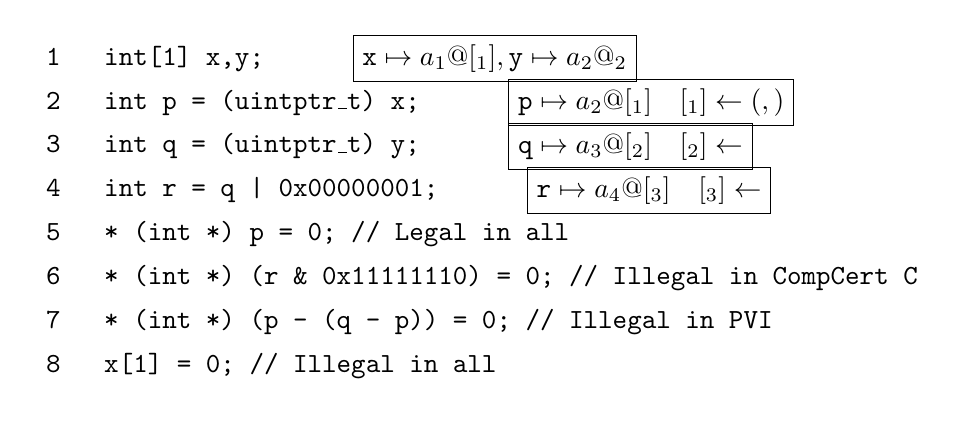
\begin{tikzpicture}[every text node part/.style={align=left}]
  \node[matrix, anchor=west] (code)
       {
         \node (l2) {\tt 1 ~ int[1] x,y;}; \\
         \node (l3) {\tt 2 ~ int p = (uintptr\_t) x;}; \\
         \node (l4) {\tt 3 ~ int q = (uintptr\_t) y;}; \\
         \node (l5) {\tt 4 ~ int r = q | 0x00000001;}; \\
         \node {\tt 5 ~ * (int *) p = 0; // Legal in all}; \\
         \node {\tt 6 ~ * (int *) (r \& 0x11111110) = 0; // Illegal in CompCert C}; \\
         \node {\tt 7 ~ * (int *) (p - (q - p)) = 0; // Illegal in PVI}; \\
         \node {\tt 8 ~ x[1] = 0; // Illegal in all}; \\
       };

  \node[right=of l2,draw,anchor=west] {\(\mathtt{x} \mapsto a_1@\pt[_1], \mathtt{y} \mapsto a_2@\pt_2\)};
  \node[right=of l3,draw,anchor=west] {\(\mathtt{p} \mapsto a_2@\vt[_1]\) ~
    \(\vt[_1] \leftarrow \picasttname(\PCT, )\)};
  \node[right=of l4,draw,anchor=west] {\(\mathtt{q} \mapsto a_3@\vt[_2]\) ~ \(\vt[_2] \leftarrow \picasttname\)};
  \node[right=of l5,draw,anchor=west] {\(\mathtt{r} \mapsto a_4@\vt[_3]\) ~ \(\vt[_3] \leftarrow \binoptname\)};
  
\end{tikzpicture}

\caption{Memory Safety and Pointer Casts}
\label{fig:memsafe}
\end{figure}

\paragraph*{Memory Safety in General}

The core of all three memory safety variants is a ``lock and key'' approach, due to
Clause et al. \cite{Clause07:MemsafeTainting} and introduced in a PIPE context in
Azevedo de Amorim et al. \cite{Azevedo+15}.
Whenever an object is allocated, it is assigned a unique ``color,'' and its memory locations as well
as its pointer are tagged with that color. The default tag \(N\) indicates that there is currently
no color. These rules are given in \cref{fig:memcommon}.
Operations that are valid on pointers in a given memory model
maintain the pointer's color, and  loads and stores are legal if the pointer tag matches the target memory
location tag.
The rules for the \(PVI\) memory safety policy are given in \cref{fig:pvi}.

\begin{figure}
  \begin{subfigure}{\textwidth}
    \begin{minipage}{0.3\textwidth}
      \color{blue}
      \begin{align*}
        \tau ::= & \clr & \clr \in \mathbb{N} \\
        & \N \\
        & \mathit{CAST} ~ \clr & \textnormal{CompCert only} \\
      \end{align*}
    \end{minipage}
    \scriptsize
    \begin{minipage}{0.3\textwidth}
      \localtruleblock
          {\(\PCT' := \PCT+1\);
            \(\pt := \PCT\)\\
            \(\vt := \N\);
            \(\lt := \PCT\)
          }
      \malloctruleblock
          {\(\PCT' := \PCT+1\);
            \(\pt := \PCT\) \\
            \(\vt := \N\);
            \(\lt := \PCT\)
          }
    \end{minipage}
    \begin{minipage}{0.3\textwidth}
      \loadtruleblock{\(\mathbf{assert} ~ \pt = \lt\) \\ \(\vt' := \vt\)}

      \storetruleblock{\(\mathbf{assert} ~ \pt = \lt\) \\
        \(\PCT' := \PCT\);
        \(\vt' := \vt\); 
        \(\lt' := \lt\)}
    \end{minipage}

    \caption{Common Memory Safety Rules}
    \label{subfig:memgen}
  \end{subfigure}
  \begin{subfigure}{0.3\textwidth}
    \color{blue}
    %
    \scriptsize
    %
    \picasttruleblock{\caseoftwo{\(\pt\)}{\(\clr\)}{\(\vt' := CAST ~ \clr\)}{\(\_\)}{\(\vt' := \pt\)}}

    \binoptruleblock{
      \caseofthree
          {\((\oplus, \vt_1,~ \vt_2)\)}
          {\((+,\clr,\N)\) \\ \((+,\N,\clr)\)}{\(\vt' := \clr\)}
          {\((\_,\N,\N)\) \\ \((-,\clr,\clr)\)}{\(\vt' := \N\)}
          {\(\underline{~ ~ ~}\)}{\(\fail\)}
    }

    \ipcasttruleblock{\caseoftwo{\(\vt[_1]\)}{\(\clr\)}{\(\vt' := CAST ~ \clr\)}{\(\_\)}{\(\vt' := \pt\)}}
    
    \caption{CompCert C Rules}
    \label{subfig:memcompcert}
  \end{subfigure}
  \begin{subfigure}{0.3\textwidth}
    \scriptsize
    
    \picasttruleblock{\(\vt' := \pt\)}

    \binoptruleblock{
      \caseofthree
          {\((\vt_1,~ \vt_2)\)}
          {\((\clr,\N)\)}{\(\vt' := \clr\)}
          {\((\N,\gentag)\)}{\(\vt' := \gentag\)}
          {\((\clr_1, \clr_2)\)}{\(\vt' := \N\)}
    }

    \ipcasttruleblock{\(\pt' := \vt\)}
    
    \caption{PVI Rules}
    \label{subfig:memcompcert}
  \end{subfigure}
  \begin{subfigure}{0.3\textwidth}
    \scriptsize
    
    \picasttruleblock{\(\vt' := \N\)}

    \binoptruleblock{
      \caseofthree
          {\((\vt_1,~ \vt_2)\)}
          {\((\clr,\N)\)}{\(\vt' := \clr\)}
          {\((\N,\gentag)\)}{\(\vt' := \gentag\)}
          {\((\clr_1, \clr_2)\)}{\(\vt' := \N\)}
    }

    \ipcasttruleblock{\(\pt' := \lt\)}
    
    \caption{PNVI Rules}
    \label{subfig:memcompcert}
  \end{subfigure}
  
    \caption{Memory Safety Rules}
    \label{fig:memcommon}
  \end{figure}

Memory safety informs our control points related to allocating, deallocating, and
accessing memory. \(\malloctname\) and \(\freetname\) are special cases of the
\(\extcalltname\) control point, which represents a call to an external function
that may tag its outputs in a specialized way.

\paragraph*{Memory Safety Variants}

Thus far we have only introduced spatial memory safety, but Tagged C also
supports temporal safety. A full memory safety policy precents use-after-free and
double-free errors by either retagging a deallocated region, or using the PC tag
to track live objects and revoking permissions on an object as soon as it is freed.

\subsection{Compartmentalization}

In a perfect world, all C programs would be memory safe. In reality, it is common
for a codebase to contain undefined behavior that will not be fixed. Developers intentionally use 
low-level idioms that are UB \cite{Memarian16:DeFacto}, or the cost and risk of regressions may make it
undesirable to fix bugs in older code \cite{Bessey10:Coverity}. Running the CompCert C or even
the PVI policy described above might break such code, while the PNVI policy might not offer enough
protection.

A compartmentalization policy can isolate potentially risky code, such as code with intentional
or unfixed UB, from safety-critical code, and enforce the {\em principle of least privilege}. 
Even in the absence of language-level errors, compartmentalization can usefully 
restrict how code in one compartment may interact with another. External libraries are
effectively required for most software to function yet represent a threat; isolating 
them from prevents vulnerabilities in the library from compromising critical code,
and limits the availability of ROP gadgets and other tools to attackers that manage to
exploit the critical code.

Let's assume that we have a compartmentalization scheme that is being added to the system
after development. A set of compartment identifiers are ranged over by \(C\),
and function and global identifiers are mapped to compartments by \(\mathit{comp}(id)\). 

\paragraph*{Compartmentalization Control Points}

Compartmentalization requires the policy to keep track of the active compartment, which means
keeping track of function pointers. In Tagged C, function pointers are the exception to the
concrete memory model. They carry symbolic values that refer uniquely to their target functions.
A variable expression where the variable is the function {\tt f} evaluates to \(\mathtt{f}@\FN[\mathtt{f}]\).
When the function pointer is called, Tagged C invokes \(\callt\), where \(\pt\) is the
function pointer's tag, to update PC tag.
On return, in addition to handling the return value (if any), \(\rett\) determines a new PC tag
based on the one before the call (\(\PCT[_{CLR}]\)) and the one at the time of return (\(\PCT[_{CLE}]\)).

In our compartmentalization policy (\cref{fig:compartments}), we define a tag to be a compartment
identifier or the default \(\N\) tag. The PC tag always carries the compartment of the
active function, kept up to date by the \(\calltname\) and \(\rettname\) rules.

\begin{figure}
  \scriptsize
  \color{blue}
  \begin{minipage}[t]{0.4\textwidth}
    \vspace{-3em}
    \[\color{blue} \tau ::= C | \N\]

    \calltruleblock{\(\PCT' := \mathit{comp}(f')\)}
  
    \rettruleblock{\(\PCT' := \PCT_{CLR};\vt':=\vt\)}
  \end{minipage}
  \begin{minipage}[t]{0.25\textwidth}
    \malloctruleblock{\(\PCT' := \PCT; \pt := \N;\) \\ \(\vt := \N; \lt := \PCT\)}
    \localtruleblock{\(\PCT' := \PCT; \pt := \N;\) \\ \(\vt := \N; \lt := \PCT\)}
  \end{minipage}
  \begin{minipage}[t]{0.25\textwidth}
    \loadtruleblock{\(\mathbf{assert} ~ \forall \lt \in \lt . \PCT = \lt\) \\ \(\vt' := \vt\)}
    
    \storetruleblock{\(\mathbf{assert} ~ \forall \lt \in \lt . \lt = \PCT\) \\
      \(\PCT' := \PCT; \vt' := \N; \lt' := \lt\)}
  \end{minipage}
    
  \caption{Simple Compartmentalization Policy}
  \label{fig:compartments}
\end{figure}

Once the policy knows which compartment is active, it must ensure that compartments do not interfere with
one another's memory. A simple means of doing so is given in \cref{fig:compmem}: any object allocated by
a given compartment, whether on the stack or via malloc, is tagged with that compartment's identity,
and can only be accessed while that compartment is active.

This is very limiting, however! In practice, compartments need to be able to share memory, such as in the
common case where libraries have separate compartments from application code. One solution is to allow
compartments to share selected objects by passing their pointers, treating them as
{\em capabilities}---unforgeable tokens of privilege.

Distinguishing shareable memory from memory that is local to a compartment is inconvenient
when the goal is to avoid modifying source code. In order to be minimally intrusive, we
create a variant identifier for {\tt malloc}, {\tt malloc\_share}, which maps to the same
address (i.e., it still calls the same function) but its name tag differs and can therefore
be used to specialize the tag rule. The need to do this is one of several limitations related
to malloc (\cref{sec:limitations}). An engineer might manually select which allocations are
shareable, or perhaps automatically using some form of escape analysis.

This policy (\cref{fig:sharing}) essentially combines the simple compartmentalization policy
and a memory safety policy.
%The PC tag carries both the current compartment color, for tagging unshared allocations, and the next free color, for tagging shared allocations.
%\(\malloctname\) uses the function tag to determine which color to attach to the pointer and allocated
%region. During loads and stores, the location tag of the target address
%determines whether access is checked via the identity of the active compartment (for unshared allocations) or
%the validity of the pointer (for shared ones).

\begin{figure}
  \color{blue}
  \scriptsize
  \begin{minipage}{0.2\textwidth}
    \[\begin{aligned}
      \tau & ::= \N \\
      & C \\
      & \clr \\
      & (C,\clr) \\
    \end{aligned}\]
  \end{minipage}
  \begin{minipage}{0.8\textwidth}
  \malloctruleblock
      {let \((C,\clr) := \PCT\) in \\
        \caseoftwo{\(\pt\)}
                  {\(\FN[\mathtt{malloc}]\)}{\(\mathbf{MallocT}_{C}(\PCT,\pt,\vt)\)}
                  {\(\FN[\mathtt{malloc\_share}]\)}
                  {\(\clr',\pt',\lt' \leftarrow \mathbf{MallocT}_{\mathit{PVI}}(\PCT,\pt,\vt)\) \\
                    & & \(\PCT':= (C,\clr');\) \\ & & \(\pt' := \pt; \vt := \N';\) \\ & & \(\lt := \clr\)}
                  
      }
  \end{minipage}
  \begin{minipage}{0.45\textwidth}
  \storetruleblock
        {let \((C,\clr) := \PCT\) in \\
          \caseoftwo{\(\lt\)}
                    {\(C'\)}{\(\mathbf{StoreT}_C(C,\N,\vt,C')\)}
                    {\(\clr'\)}{\(\mathbf{StoreT}_{\mathit{PVI}}(\clr,\pt,\vt,\clr')\)}}

  \end{minipage}
  \begin{minipage}{0.3\textwidth}
    \loadtruleblock
        {let \((C,\clr) := \PCT\) in \\
          \caseoftwo{\(\lt\)}
                    {\(C'\)}{\(\mathbf{StoreT}_C(C,\N,\vt,C')\)}
                    {\(\clr'\)}{\(\mathbf{StoreT}_{\mathit{PVI}}(\clr,\pt,\vt,\clr')\)}}
  \end{minipage}

  
  \caption{Compartmentalization with Shared Capabilities}
  \label{fig:sharing}
\end{figure}

\paragraph*{Compartmentalization Variants}

Using program-specific tags for globals and functions, a compartmentalization policy
like the one above can be extended with a Mandatory Access Control (MAC) policy.

\subsection{Secure Information Flow}

Our final example policy will expand on our example of
{\em secure information flow} (SIF)~\cite{Denning77:SecureInformationFlow}.
This family of policies deal entirely with enforcing
higher-level security concerns, regardless of whether the code that they protect contains
errors or undefined behaviors.

\begin{figure}
\begin{tikzpicture}[every text node part/.style={align=left}]
  \node[matrix, ampersand replacement=\&, anchor=west] (code)
       {
         \node {\tt 1 void h(int id, int psk) \{}; \\
         \node (l1) {\tt 2 ~ int fmt = check\_format(psk);}; \\
         \node (l2) {\tt 3 ~ switch(format(psk)) \{}; \\
         \node {\tt 4 ~ ~ case OLD:}; \\
         \node {\tt 5 ~ ~ ~ psk = update(psk); break;}; \\
         \node {\tt 6 ~ ~ case INVALID:}; \\
         \node {\tt 7 ~ ~ ~ psk = 0; break;}; \\
         \node {\tt 8 ~ ~ case DEFAULT:}; \\
         \node {\tt 9 ~ \}}; \\
         \node (l3) {\tt 10 J:  printf("Updating user \%d", id); // join point}; \\
         \node {\tt 11 ~ update(id, psk);}; \\
         \node {\tt 12 \}}; \\
       };

    \node[matrix, ampersand replacement=\&, node distance=12em, right=of l2.north,draw] (table1)
         {
           \node[anchor=north] {\(h@\PCT[_1]\)};\\
         };

    \node[matrix, ampersand replacement=\&, node distance=4.5em, below=of table1.west,draw,anchor=west] (table2)
         {
           \node[anchor=north] {\(h@\PCT[_3]\)}; \&
           \node[anchor=north] {\(\PCT[_2], \vt[_1] \leftarrow \rettname(\dots)\) \\
             \(\PCT[_3] \leftarrow \splittname(\PCT[_2], \vt_1)\) }; \\
         };

    \node[matrix, ampersand replacement=\&, node distance=4.5em, below=of table2.west,draw,anchor=west] (table3)  
         {
           \node[anchor=north] {\(h@\PCT[_4]\)}; \&
           \node[anchor=north] {\(\PCT[_4] \leftarrow \labeltname(\PCT[_3], \LN[J])\)}; \\
         };

    \draw[Circle-]
    (l1.south) -- (table1.west);

    \draw[Circle-]
    (l2.south) -| (table2.north);

    \draw[Circle-]
    (l3.north) |- (table3.west);  

\end{tikzpicture}
\caption{Not an Implicit Flow}
\label{fig:sifex3}
\end{figure}

In \cref{fig:sifex3}, the program checks the format of the passkey, and uses a switch statement to perform
operations on it based on the result. As we saw back in \cref{fig:ex2}, this means that the policy
should ``raise'' the PC tag to represent that the program's control-flow depends on {\tt psk}.
But in \cref{fig:sifex3}, after the branches of the switch statement have completed, this is no
longer necessary---no information can be gleaned from the store to {\tt psk} once execution has
reached label {\tt J}. {\tt J} is a {\em join point}: the point in a control-flow graph where all
possible routes from the split to a return have re-converged, which can be identified
statically as the immediate post-dominator of the split point \cite{Denning77:SecureInformationFlow}.

In order to support policies that reason about splits and joins, we introduce the \(\splittname\),
\(\exprsplittname\), \(\labeltname\), and \(\exprjointname\) tag rules. Every transition that tests a
value as part of a conditional or loop contains a control point that calls \(\splittname\), with an
optional label that is part of Tagged C's abstract syntax. This way, the policy can react when execution
reaches that label via the \(\labeltname\) rule. In the full SIF policy, we will keep track of
the pending join point on the PC tag, and lower the PC tag when execution reaches the join point.
A similar structure applies to conditional expressions, except that the policy doesn't need to track
an arbitrary label: \(\exprjointname\) always triggers when a conditional expression is fully evaluated.

\begin{figure}
  \begin{minipage}{0.3\textwidth}
    \color{blue}
    \begin{align*}
      \tau ::= & \high \\
      & \low \\
      & \pctaint{f}{d}{Ls} & d \in \mathbb{N}, ~ Ls \in \mathit{list} ~ id \\
    \end{align*}
  \end{minipage}
  \begin{minipage}{0.69\textwidth}
    \[|\gentag| \triangleq
    \begin{cases}
      \low & \textnormal{if } \gentag = \low \textnormal{ or } \gentag = \pctaint{f}{0}{\varepsilon} \\
      \high & \textnormal{otherwise} \\
    \end{cases}\]
    %
    \[\gentag_1 \sqcup \gentag_2 \triangleq
    \begin{cases}
      \low & \textnormal{if } |\gentag_1| = |\gentag_2| = \low \\
      \high & \textnormal{otherwise} \\
    \end{cases}\]
  \end{minipage}
  \begin{minipage}{0.55\textwidth}
    \splittruleblock{
      \caseoftwo{\(\PCT, \vt\)}
                {\(\pctaint{f}{d}{Ls}, \low\)}{\(\PCT' := \pctaint{f}{d}{(L::Ls)}\)}
                {\(\underline{~~~}, \high\)}{\(\PCT' := \PCT\)}
    }
    \labeltruleblock{
      \caseoftwo{\(\PCT\)}
                {\(\pctaint{f}{d}{Ls}\)}{
                  let \({\color{blue} Ls'} = \mathit{pop\_all} ~ {\color{blue} \LN ~ Ls}\) in \\
                  & &      \(\PCT' := \pctaint{f}{d}{Ls'}\)
                }
                {\(\underline{~~~}\)}{\(\PCT' := \PCT\)}
    }
  \end{minipage}
  \begin{minipage}{0.35\textwidth}
    \exprsplittruleblock{
      \caseoftwo{\(\PCT, \vt\)}
                {\(\pctaint{f}{d}{Ls}, \low\)}{\(\PCT' := \pctaint{f}{(d+1)}{Ls}\)}
                {\(\underline{~~~}, \high\)}{\(\PCT' := \PCT\)}
    }

    \exprjointruleblock{
      \(\vt' := \vt \sqcap \PCT\) \\
      \caseoftwo{\(\PCT\)}
                {\(\pctaint{f}{(d+1)}{Ls}\)}{\(\PCT' := \pctaint{f}{d}{Ls}\)}
                {\(\underline{~~~}\)}{\(\PCT' := \PCT\)}
    }
  \end{minipage}
  
  \caption{SIF Conditionals}
  \label{fig:SIFconditionals}
\end{figure}

In addition to \(\low\) and \(\high\), the SIF policy tracks a PC tag written using the
constructor {\sc \color{blue} pc}, which carries (1) the current function identifier,
(2) a natural number to record a count of tainted expression scopes, and (3) a stack of label
identifiers to record the join points of tainted statement scopes.
Initial, the PC tag is \(\pctaint{f}{0}{\varepsilon}\), which intuitively corresponds
to ``low'' security. The reduce operator, \(| \cdot |\), maps this tag into \(\low\)
and a PC tag with any pending contexts into \(\high\). The join operator, \(\cdot \sqcup \cdot\),
takes the higher of its arguments after reducing them.

In order to use this version of SIF, the program must undergo a transformation introducing
the labels of all join points explicitly, so that {\tt J} is an explicit label in the code,
if it wasn't already. This is a relatively minor transformation, and is necessary because,
in the presence of go-to, break, and continue statements, the join point of a conditional might be
arbitrarily removed from it. The internal syntactic form of each conditional statement
(if, switch, while, do-while, and for) takes this optional label, and if
the conditional branches on a high value, \(\splittname\) pushes the label to the stack
in the PC tag. Later, when execution reaches a label, \(\labeltname\) checks if it is the
top of the join-point stack and deletes it if so.

For branching expressions, if \(\exprsplittname\) is invoked with \(\vt = \high\),
or if the expression counter on the PC tag is non-zero, it increments the counter.
\(\exprjointname\) decrements the counter, and when it reaches zero, we know that
control has moved past the original high context.
\apt{What is the reason for joining with P for the value?}
\sna{The result of the expression is going to be tainted by its control flow.}

\paragraph*{SIF Variants}

SIF can cover a wide array of different policies. Here we have shown an instance of
a confidentiality policy, but it can also support integrity
(``insecure inputs do not affect secure data''), intransive policies
(``data can flow from A to B and B to C, but not from A to C,'') and policies with
more than two security levels.

We have sketched a few instances of practical SIF policies. An intransitive integrity policy
can be used to protect against SQL Injections by requiring unsafe inputs to pass through a sanitizer
before they can be appended to a query. Similarly, a more complex SIF policy could ensure that
data at rest is always encrypted, by setting a low security level to the outputs of an encryption
routine and a high level to the outputs of its corresponding decryption routine.
%      As SIF, with special rule for sanitization function \\  
%      & Guarantee Encrypted Data at Rest by requiring all stores to first pass through an encryption routine &
%      As SIF, with special rules for encryption and decryption functions \\ 

\section{Evaluation}
\label{sec:evaluation}

Tagged C aims to combine the flexibility of tag-based architectures with the abstraction
of a high-level language. In the last section, we demonstrated three classes of policies
with broad practical applicability and described how they can be tuned to the needs of a
particular program. They can be used alone or in conjunction.

Additionally, the Tagged C semantics support the full complement of C language features and
give definition to many undefined C programs

% Trying to just thread the table into each section rather than all at once
%\begin{table}
%  \begin{center}
%    %\begin{tabular}{ c| c |c }
%    \title{Further Policies and their Uses}
%    \begin{tabular}{  p{3cm} | p{5cm}| p{5cm}  } 
%      \textbf{Name} & \textbf{Example Use Cases} & \textbf{Tag Implementation} \\ 
%      \hline
%      SIF: Intransitive Integrity &
%      Protect agains SQL Injection by requiring outside data to pass through a sanitizer &
%      As SIF, with special rule for sanitization function \\  
%      & Guarantee Encrypted Data at Rest by requiring all stores to first pass through an encryption routine &
%      As SIF, with special rules for encryption and decryption functions \\ 
%      Temporal Memory Safety & Prevent double free & Assign unique color to tag at each free. Check for an existi%ng color before freeing. \\
%      & Prevent Use-after-free & Check pointers for color tag when dereferencing pointers  \\
%      Placeholder-name & Placeholder-use case & Placeholder policy \\
%      \hline
%    \end{tabular}
%  \end{center}
%\end{table}
  
\subsection{Limitations}
\label{sec:limitations}

By committing to a tag-based mechanism, we do restrict the space of policies that Tagged C
can enforce. In general, a reference monitor can enforce any policy that constitutes a
{\em safety property}---any policy whose violation can be demonstrated by a single finite
trace. Some policies in this class cannot be enforced effectively by a tag-based monitor,
because tags can carry information about the provenance of values but not about the values
themselves: this rules out policies such as ``no integer overflow'' and
``pointers are always in-bounds.'' As we have seen, there are plenty of useful policies that
engage only with the provenance of values. For such policies, tag-based enforcement is
also conceptually close to the trace-based definition: defining e.g. memory safety in terms
of normal states requires either manually keeping track of large amounts of history to
identify where each pointer comes from, or possibly some sort of temporal logic.

The other known limitation is in how we tag memory at allocation time. Malloc tags an
entire region with a single tag, which means that Tagged C cannot easily
enforce substructural memory safety and other properties that call for allocated
regions to be tagged according to their types. We would rather be able to tag the allocated region
based on its type, but in C, malloc does not get access to type information---it allocates
memory of a given side and returns a {\tt void *}, and it is up to the caller to cast the
pointer to the desired type. That cast may be arbitrarily removed from the call to malloc!
This is not just a problem in the Tagged C context; Michael et al.
\cite{Michael23:MSWASM} approach a similar problem by outright replacing {\tt malloc}
with a {\tt segalloc} function that takes much more information.
Versions of memory safety that protect fields of a
struct from overflows within the same struct would be very useful, but currently enforcing
them will require manual initialization.

Beyond these, there is always the possibility that we have missed some control point
that would enable interesting security policies outside of the areas we have considered.
How hard would it be to add control points, or extend the ones that exist? That depends
whether the extension in question would impact compilation strategies. For instance,
we have avoided control points that allow updates to their operand tags, although
this could be useful in enforcing policies that attempt to maintain the uniqueness of tags,
because tag-based hardware is unlikely to support linear tags, so any such updates would
need the compiler to generate extra instructions.

\section{Related Work}
\label{sec:related}

\paragraph{Reference Monitors}

The concept of a reference monitor was first introduced fifty years ago~\cite{Anderson72:PlanningStudy}
as a tamper-proof and verifiable subsystem that checks every security-relevant operation in a system to
ensure that it conforms to a security {\em policy} (a general specification of acceptable behavior~\cite{Goguen82:SecurityPolicies}).

A reference monitor can be implemented at any level of a system. An {\em inline reference monitor}\cite{??}
is a purely compiler-based system that inserts checks at appropriate places in the code.
Alternatively, a reference monitor might be embedded in the operating system, or in an interpreted
language's runtime. A {\em hardware reference monitor} instead provides primitives at the ISA-level
that accelerate security and make it harder to subvert.

Programmable Interlocks for Policy Enforcement (PIPE) \cite{Dhawan14:PUMP} is a hardware extension
that uses {\em metadata tagging}. Each register and each word of memory is associated with
an additional array of bits called a tag. The policy is decomposed into a set of {\em tag rules}
that act in parallel with each executing instruction, using the tags on its operands to
decide whether the instruction is legal and, if so, determine which tags to place on its results.
PIPE tags are large relative to other tag-based hardware, giving it the flexibility
to implement complex policies with structured tags, and even run multiple policies at once.

Other hardware monitors include Arm MTE, STAR, and CHERI.
Arm MTE aims to enforce a narrow form of memory safety using 4-bit tags, which distinguish adjacent objects
in memory from one another, preventing buffer overflows, but not necessarily other memory violations.
[TODO: read the Binghamton paper, figure out where they sit here.] 

CHERI is capability machine [TODO: cite OG CHERI]. In CHERI, capabilities
are ``fat pointers'' carrying extra bounds and permission information, and capability-protected
memory can only be accessed via a capability with the appropriate privilege. This is a natural
way to enforce spatial memory safety, and techniques have been demonstrated for enforcing
temporal safety \cite{NWF20:Cornucopia}, stack safety \cite{Skorstengaard19:stktokens},
and compartmentalization [TODO: figure out what to cite], with varying degrees of ease and
efficiency. But CHERI cannot easily enforce notions of security based on dataflow,
such as Secure Information Flow.

In this paper, we describe a programming language with an abstract reference monitor.
We realize it as an interpreter with the reference monitor built in, and envision
eventually compiling to PIPE-equipped hardware, although an inlining compiler would also be plausible.
This motivates many of our assumptions about tags.

%\paragraph{Aspect Oriented Programming}
%[TODO: do forward search from original AOP paper]

\section{Future Work}
\label{sec:futurework}

We have presented the language and a reference interpreter, built on top of the CompCert interpreter
\cite{Leroy09:CompCert}, and three example policies. There are several significant next-steps.

\paragraph{Compilation}

An interpreter is useful for testing, but a compiler would be preferable for many reasons.
A compiled Tagged C could use the hardware acceleration of a PIPE target, and could more easily
support linked libraries, including linking against code written in other languages.
The ultimate goal would be a fully verified compiler.

\paragraph{Language Proofs}

There are a couple of properties of the language semantics itself that we would like to prove.
Namely (1) that its behavior (prior to adding a policy) matches that of CompCert C and
(2) that the behavior of a given program is invariant under all policies up to truncation due
to failstop.

\paragraph{Policy Correctness Proofs}

For each example policy discussed in this paper, we sketched a formal specification for the
security property it ought to enforce. A natural continuation would be to prove the correctness
of each policy against these specifications.

\paragraph{Policy DSL}

Currently, policies are written in Gallina, the language embedded in Coq. This is fine for a
proof-of-concept, but not satisfactory for real use. We plan to develop a domain-specific policy
language to make it easier to write Tagged C policies.

\bibliographystyle{splncs04}
\bibliography{taggedc.bib}

\appendix

\section{Syntax}

Tagged C has the full complement of typical C expressions (\cref{fig:expr}). \(\val{v}{\vt}\),
\(\loc{p}{\pt}\), and \(\paren{\expr}{\type}\) are internal forms.
A constant \(c\) in the concrete syntax is transformed into \(\val{c}{\constt}\),
and in general \(\val{v}{\vt}\) is a fully-reduced right-hand value. \(\loc{p}{\pt}\)
is a fully-reduced left-hand value that represents the address of a variable.
\(\paren{\expr}{\type}\) is the result of a conditional or shortcutting
expression, with \(\type\) being a type annotation in case the result needs to
be cast.

\begin{figure}
  \[\begin{aligned}
  \expr ::= & \val{v}{\vt} & \textnormal{Value} \\
  | & \var{x} & \textnormal{Variable} \\
  | & \field{\expr}{id} & \textnormal{Field} \\
  | & \valof{\expr} & \textnormal{Load from Object} \\
  | & \deref{\expr} & \textnormal{Dereference Pointer} \\
  | & \addrof{\expr} & \textnormal{Address of Object} \\
  | & \unop{\odot}{\expr} & \textnormal{Unary Operator} \\
  | & \binop{\oplus}{\expr_1}{\expr_2} & \textnormal{Binary Operator} \\
  | & \cast{\expr}{ty} & \textnormal{Cast} \\
  | & \condition{\expr_1}{\expr_2}{\expr_3} & \textnormal{Conditional} \\
  | & \sizeof{ty} & \textnormal{Size of Type} \\
  | & \alignof{ty} & \textnormal{Alignment of Type} \\
  | & \assign{\expr_1}{\expr_2} & \textnormal{Assignment} \\
  | & \assignop{\oplus}{\expr_1}{\expr_2} & \textnormal{Operator Assignment} \\
  | & \postinc{\oplus}{\expr} & \textnormal{Post-Increment/Decrement} \\
  | & \comma{\expr_1}{\expr_2} & \textnormal{Expression Sequence} \\
  | & \call{\expr_f}{\overline{\expr}_{args}} & \textnormal{Function Call} \\
  | & \loc{l}{\lt} & \textnormal{Memory Location} \\
  | & \paren{\expr}{ty}{\gentag} & \textnormal{Parenthetical with Optional Cast} \\
  \end{aligned}\]
  \caption{Expression Syntax}
  \label{fig:expr}
\end{figure}

Some common C expressions are derived forms. An array index expression,
\(\expr_1[\expr_2]\) expands to \(\deref{\binop{+}{\expr_1}{\expr_2}}\).
The pre-increment  expression \(++\expr\) expands to
\(\assign{\expr}{\binop{+}{\expr}{1@\constt}}\), and likewise for pre-decrement.

Similarly, statements cover the full C standard. Conditional statements
carry optional labels as internal forms, so that an if statement in the
concrete syntax becomes \(\sifthenelse{\expr}{\stmt_1}{\stmt_2}{\bot}\).

\begin{figure}
  \begin{subfigure}[t]{0.3\textwidth}
    \[\begin{aligned}
    \stmt ::= & \sskip \\
    | & \sdo{\expr} \\
    | & \sseq{\stmt_1}{\stmt_2} \\
    | & \sifthenelse{\expr}{\stmt_1}{\stmt_2}{L} \\
    | & \swhile{\expr}{\stmt}{L} \\
    | & \sdowhile{\expr}{\stmt}{L} \\
    | & \sfor{\stmt_1}{\expr}{\stmt_2}{\stmt_3} \\
    | & \sbreak \\
    | & \scontinue \\
    | & \sreturn \\
    | & \sswitch{\expr}{\overline{(L,\stmt)}} \\
    | & \slabel{L}{\stmt} \\
    | & \sgoto{L} \\    
    \end{aligned}\]
  \end{subfigure}
  \begin{subfigure}[t]{0.69\textwidth}
  \end{subfigure}
  \caption{Tagged C Abstract Syntax}
  \label{fig:syntax}
\end{figure}

\section{States}

States can be of several kinds, denoted by their script prefix: a {\em general state} \(\mathcal{S}(\dots)\),
an {\em expression state} \(\mathcal{E}(\dots)\), a {\em call state} \(\mathcal{C}(\dots)\), or a
{\em return state} \(\mathcal{R}(\dots)\). Finally, the special state {\em failstop} (\(\mathcal{F}(\dots)\))
represents a tag failure, and carries the state that produced the failure.
[Allison: to whatever degree you've figured out what is useful here by publication-time, we can
  tune this to be more specific.]

In the below definition, memories are ranged over by \(\mem\), local environments by
\(\lenv\), and continuations by \(\cont\).

\[\begin{aligned}
S ::= & \sstate{\PCT}{\mem}{\stmt}{\cont} \\
| & \estate{\PCT}{\mem}{\expr}{\cont} \\
| & \cstate{f}{\PCT}{\mem}{\lenv}{f'}{\overline{\val{v}{\vt}}}{\cont} \\
| & \rstate{\PCT}{\mem}{\genv}{\lenv}{\val{v}{\vt}}{\cont} \\
| & \fstate{S} \\
\end{aligned}\]


States in general contain a memory, a local environment, and a continuation.

\subsection{Memories}

\subsection{Environments}

\subsection{Continuations}
\label{app:continuations}

A continuation acts like a stack of pending operations. The base of the stack is
\(\kemp\). \(\mathit{Kdo}\) indicates that a do statement is evaluating an expression.
\(\mathit{Kseq}\) with parameter \(\stmt\) indicates that, after the current statement
is done executing, \(\stmt\) is next. \(\mathit{Kif}\) means that execution is evaluating
the test expression of an if statement, and its parameters are the branches of the
if. Similarly, the test continuations for while, do-while, and for loops indicate that
the test expression is being evaluated. The associated loop continuations indicate that
execution is in the loop body. They continuations carry all of the information of the original
loop.

\[\begin{split}
\cont ::= & \kemp \\
| & \kdo{\cont} \\
| & \kseq{\stmt}{\cont} \\
| & \kif{\stmt_1}{\stmt_2}{L}{\cont} \\
| & \kwhiletest{\expr}{\stmt}{L}{\cont} \\
| & \kwhileloop{\expr}{\stmt}{L}{\cont} \\
| & \kdowhiletest{\expr}{\stmt}{L}{\cont} \\
| & \kdowhileloop{\expr}{\stmt}{L}{\cont} \\
| & \kfor{\expr}{\stmt_2}{\stmt_3}{L}{\cont} \\
| & \kforpost{\expr}{\stmt_2}{\stmt_3}{L}{\cont} \\
\end{split}\]


\section{Initial State}

Given a list \(xs\) of variable identifiers \(id\) and types
\(ty\), a program's initial memory is defined by iteratively allocating each one
in memory and updating the global environment with its base address, bound, type,
and a static identity tag. Let \(|ty|\) be a function from types to their sizes
in bytes. The memory is initialized \(\vundef@\vt@\lt\)
for some \(\vt\) and \(\lt\), unless given an initializer.
Let \(\mem_0\) and \(\genv_0\) be the initial (empty) memory and environment.
The parameter \(b\) marks the start of the global region.

%Since we don't need to initialize tags in memory dynamically, our rule for
%selecting these tags can cover the entire initialization of the memory with arbitrary
%granularity. We represent this as a list of tags of length \(|ty|\).

\[\mathit{globals} ~ xs ~ b =
\begin{cases}
  (\mem_0, \genv_0) & \textnormal{if } xs = \varepsilon \\
  (\mem[p \dots p+|ty| \mapsto \vundef@\vt@\lt]_{|ty|}, & \textnormal{if } xs = (id,ty)::xs' \\
  ~ \genv[id \mapsto (\mathit{p, p+|ty|,ty,\pt})]) & \textnormal{and } \trule{\globaltres}{\globalt} \\
  & \textnormal{where } (\mem,\genv) = \mathit{globals} ~ xs' ~ (b + |ty|) \\
\end{cases}\]

\section{Step Rules}
\label{app:rules}

\subsection{Sequencing rules}

\sequencing

\subsection{Conditional rules}

\conditionals

\subsection{Loop rules}

\loops

\subsection{Contexts}
\label{app:contexts}

Our expression semantics are contextual. A context \(\ctx[\expr]_k\) is a function from an
expression to an expression, with a ``kind'' flag \(k\) (left-hand or right-hand, \(\lh\) or \(\rh\)).

\[\begin{aligned}
\ctx{\expr}_\lh ::= \\
| & \expr & \\ % ctx_top
| & \deref{\ctx{\expr}_\rh} \\ % ctx_deref
| & \field{\ctx{\expr}_\rh}{id} \\ % ctx_field
\end{aligned}\]

\[\begin{aligned}
\ctx{\expr}_\rh ::= \\
| & \expr & \\ % ctx_top
| & \valof{\ctx{\expr}_\lh} \\ % ctx_rvalof
| & \addrof{\ctx{\expr}_\lh} \\ % ctx_addrof
| & \unop{\odot}{\ctx{\expr}_\rh} \\ % ctx_unop
| & \binop{\oplus}{\ctx{\expr_1}_\rh}{\expr_2} \\ % ctx_binop_left
| & \binop{\oplus}{\expr_1}{\ctx{\expr_2}_\rh} \\ % ctx_binop_right
| & \cast{\ctx{\expr}_\rh}{\type} \\ % ctx_cast
| & \seqand{\ctx{\expr_1}_\rh}{\expr_2} \\ % ctx_seqand
| & \seqor{\ctx{\expr_1}_\rh}{\expr_2} \\ % ctx_seqor
| & \condition{\ctx{\expr_1}_\rh}{\expr_2}{\expr_3} \\ % ctx_condition
| & \assign{\ctx{\expr_1}_\lh}{\expr_2} \\ % ctx_assign_left
| & \assign{\expr_1}{\ctx{\expr_2}_\rh} \\ % ctx_assign_right
| & \assignop{\oplus}{\ctx{\expr_1}_\lh}{\expr_2} \\ % ctx_assignop_left
| & \assignop{\oplus}{\expr_1}{\ctx{\expr_2}_\rh} \\ % ctx_assignop_right
| & \postinc{\oplus}{\ctx{\expr}_\lh} \\ % ctx_postinc
| & \call{\ctx{\expr_1}_\rh}{\overline{\expr_2}} \\ % ctx_call_left
| & \call{\expr_1}{\ctx{\overline{\expr_2}}_\rh} \\ % ctx_call_right
% skipped builtins
| & \comma{\ctx{\expr_1}_\rh}{\expr_2} \\ % ctx_comma
| & \paren{\ctx{\expr}_\rh}{\type}{} \\ % ctx_paren
\end{aligned}\]

A left-hand reduction \(\expr \Rightarrow_\lh \expr'\)
relates an expression to an expression. A right-hand reduction
\((\PCT,\mem,\expr) \Rightarrow_\rh (\PCT',\mem',\expr')\)
relates a triple of PC Tag, memory, and expression to another such triple.
Given these reduction relations, we construct step rules for contexts in
expressions.

%triple of a memory, an expression, and a tag
%might reduces to another such triple as a left-hand, right-hand, or call reduction, written
%\((\mem, \expr, \PCT) \Rightarrow_k (\mem', \expr', \PCT')\),
%based on rules given below. These reductions are embedded in states as follows.

\judgmenttwo{\(\ctx{\expr}_\lh\)}
            {\(\expr \Rightarrow_\lh \expr'\)}
            {\(\defestate{\ctx{\expr}} \longrightarrow \defestate{\ctx{\expr'}}\)}

\judgmenttwo{\(\ctx{\expr}_\rh\)}
            {\((\PCT, \mem, \expr) \Rightarrow_\rh (\PCT', \mem', \expr')\)}
            {\(\defestate{\ctx{\expr}} \longrightarrow \estate{\PCT'}{\mem'}{\ctx{\expr'}}{\cont}\)}
            
All that remains is to give the expression reductions themselves.

\expressions

\subsection{Call and Return Rules}

In order to make a call, we need to reduce the function expression to an \(\floc{\_}\) value, an
abstract location corresponding to a particular function. Then we can make the call.

\callexprstep

When we make an internal call, we need to allocated space for locals and arguments using the helper function
\(\mathit{frame}\).

\[\mathit{frame} ~ xs ~ as ~ \mem =
\begin{cases}
  (\mem''[p \mapsto \vundef@\vt@\lt]_{|ty|}, & \textnormal{if } xs = (id,ty)::xs' \\
  \lenv'[id \mapsto (\mathit{p, p+|ty|,ty,\pt})]) &
  \textnormal{where } (\mem',p) \leftarrow \mathit{stack\_alloc} ~ |ty| ~ \mem, \\
  & \trule{\localtres}{\localt}, \\
  & \textnormal{and } (\mem'',\lenv') = \mathit{frame} ~ xs' ~ as ~ m' \\ 
  \\
  (\mem''[p \mapsto v@\vt'@\lt]_{|ty|}, & \textnormal{if } as = (id,ty,v @ \vt)::as' \textnormal{ and } xs = \varepsilon \\
  \lenv'[id \mapsto (\mathit{p, p+|ty|,ty,\pt})]) &
  \textnormal{where } (\mem',p) \leftarrow \mathit{stack\_alloc} ~ |ty| ~ \mem, \\
  & \trule{\argtres}{\argt}, \\
  & \textnormal{and } (\mem'',\lenv') = \mathit{frame} ~ xs' ~ as ~ m' \\
  \\
  (\mem, \lambda x . \bot) & \textnormal{if } xs = \varepsilon \textnormal{ and } as = \varepsilon \\
\end{cases}\]

\callstep

On the other hand, when we make an external call, we step directly to a return state with some value
being returned and an updated memory. [TODO: talk more about how the tag policy applies in external
  functions, what they can and can't do with tags.]

\extcallstep

Special external functions, such as malloc, just get their own rules.

\mallocstep

And finally, we have the return rules.

\returnstep
\retvalstep
\retnovalstep

%\section{Moved from Intro}

%\sna{I'm organizing our diss tracks into paragraphs that we can cut or move as needed}
%\paragraph*{Why Dynamic?}
  
%  Unfortunately, it is not always possible to fully secure C code before run-time.
%  Ideally, bugs would be quickly identified and then fixed promptly. 
%  That is not always possible for a variety of reasons: bugs may escape detection, 
%  require significant effort to diagnose, or be impractical to fix. 
%  There are many techniques for finding bugs, but there is a shared stumbling block: C is not 
%  well defined. We cannot always agree on when something is a bug in C, especially code using
%  Undefined Behaviors (UB) \cite{defactoC}. Confusion around expected behavior is no small problem. 
%  There are 191 undefined behaviors and 52 unspecified behaviors in the C99 
%  specification \cite{Csmith}. Sometimes these behaviors are benign and skillfully 
%  used by the developer, other times they are unintended and highly dangerous. 
%  Unfortunately the distinction between the two is easily lost. 
%  Discerning expert code review is considered best practice, although it is 
%  rarely perfectly successful \cite{} % https://dl.acm.org/doi/10.1007/978-3-642-36563-8_14 }
%  even if an expert is available at all. Even when there is both consensus 
%  and detection of a bug\apt{??} \amn{we can find it at and we can agree its a problem that should be fixed}, 
%  changing the code may not be possible because  
%  it is in proprietary 3rd party libraries and drivers, or because
%  regulations prohibit changes \cite{Bessey10:Coverity}.

%  \apt{last clause is mysterious} \amn {
%    for example FDA approval used to forbid patching because you'd have to go through recertification. 
%    So healthcare wouldn't patch. SNA pointed out the coverity paper comments on this as a reason for 
%    bugs not getting fixed}

%  \paragraph*{Why C-Level?}
%  Tag-based enforcement in general has a significant body of work at the assembly level, especially
%  PIPE (Programmable Interlocks for Policy Enforcement) \cite{}. However, even at the assembly-level
%  these systems need the compiler to be in the trusted computing base (TCB), as many policies require
%  knowledge of source-level constructs, even ones that do not depend on detailed knowledge of the program's
%  behavior [cite Nick and Andre; anyone else?]. Moving policy-definition to the source level therefore
%  does not expand the TCB and allows C developers to reason about policies in terms of the language that
%  they program in regularly.

%  \paragraph*{Notations}
%  Values are ranged over by \(v\), variable identifiers by \(x\), and function identifiers by \(f\).
%Tags use a number of metavariables: \(t\) ranges over all tags, while we will use
%\(\vt\) to refer to the tags associated with values, \(\pt\) for tags on pointer values
%and memory-location expressions, \(\lt\) for tags associated with memory locations themselves,
%\(\nt\) for ``name tags'' automatically derived from identifiers, \(\PCT\) for the
%global ``program counter tag'' or PC tag.
%An {\it atom} is a pair of a value and a tag, \(\val{v}{\vt}\); the @ symbol should be read
%as a pair in general, and is used when the second object in the pair is a tag.
%Expressions are ranged over by \(\expr\), statements by \(\stmt\), and continuations by \(\cont\).
%The continuations are defined in \cref{app:continuations}, and step rules in \cref{app:rules}.

%A memory is an array of bytes, where each byte is part of an atom.
%Each byte is also associated with a ``location tag'' \(\lt\). When a contiguous region of \(s\) bytes
%starting at location \(l\) comprise an atom \(v@\vt\), and their locations tags comprise the list \(\lts\),
%we write \(\mem[l]_s = v@\vt @\lts\). Likewise, \(\mem[l \dots l + s \mapsto v@\vt @ \lts]_s\)
%denotes storing that many bytes. Visually, we will represent whole atoms in memory as condensed boxes,
%with their location tags separate.

\end{document}
